\section{Визуализация протокола исправления ошибок Cascade}
Программа Cascade разрабатывалась позже, чем Requc, что позволило учесть некоторые особенности визуализаций процессов и создать более четкую архитектуру.
В Cascade также используется шаблон MVVM. Схема классов Моделей и Моделей Представления изображена на рисунке \ref{fig:cascade_models}.
\begin{figure}[h]
  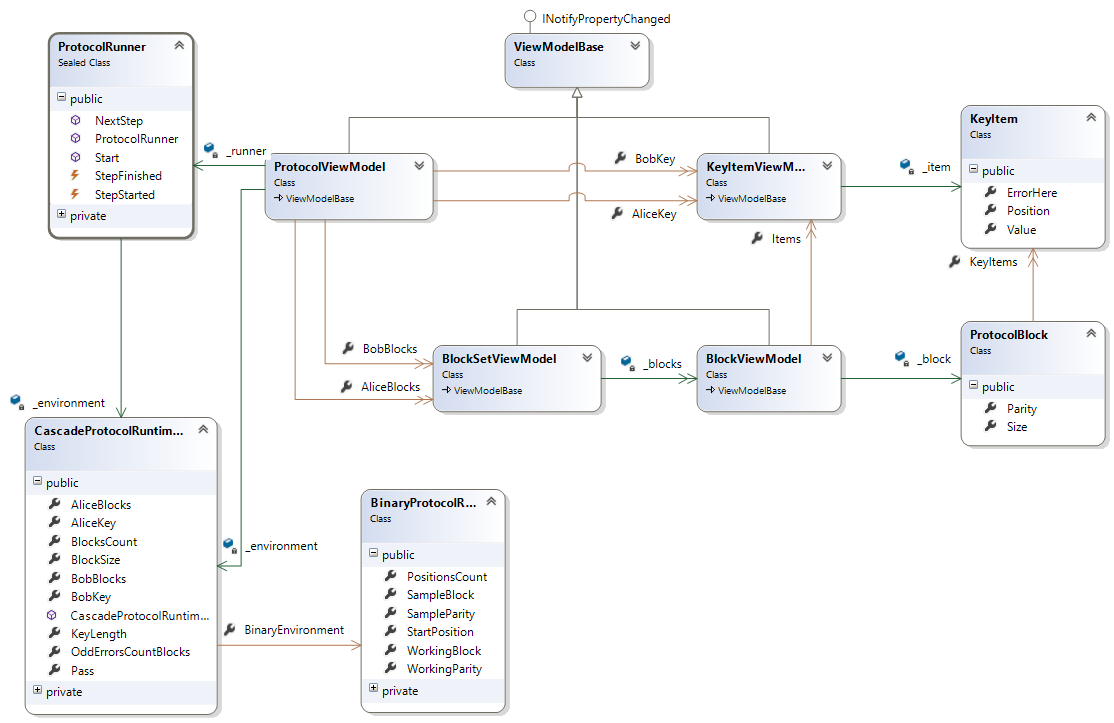
\includegraphics[width=0.9\linewidth]{chapter3/cascade_models}
  \caption{Диаграмма классов программы Cascade.}
  \label{fig:cascade_models}
\end{figure}

Некоторые пояснения к схеме классов. В центре собраны Модели Представлений, по краям схемы классы Моделей.
Основная используемая сущность~--- \mintinline{csharp}{KeyItem}, представляющая собой бит ключа Алисы или Боба.
В процессе работы протокола \ref{sec:cascade_description} ключ разбивается на блоки, которые представляются в программе экземплярами класса \mintinline{csharp}{ProtocolBlock}.

На каждый созданный блок ссылается один из экземпляров Модели Представления \mintinline{csharp}{BlockViewModel}. Набор \mintinline{csharp}{BlockViewModel} содержится в классе \mintinline{csharp}{BlockSetViewModel}, что представляет собой набор блоков на одном из проходов. 

Основную работу делает \mintinline{csharp}{ProtocolRunner}. Именно он производит необходимые действия над рабочим окружением~--- \mintinline{csharp}{CascadeProtocolRuntimeEnvironment}, которое содержит в себе всю актуальную на текущий момент информацию о ключах Алисы и Боба. \mintinline{csharp}{BinaryProtocolRuntimeEnvironment} создается каждый раз, когда приходится исправлять ошибку бинарным поиском.

\mintinline{csharp}{ProtocolRunner} создает отдельный поток, работающий в фоновом режиме и отправляющий в основной поток информацию о процессе выполнения. Каждое изменение состояния окружения должно быть визуализировано, поэтому этот фоновый процесс по завершению каждого шага останавливается и ждет разрешения продолжить выполнение. Это разрешение выдается сразу, как только все Представления сообщили, что закончили свои анимации. 

Работа состоит из набора шагов. Шагом называется элементарное действие или набор таких действий, связанных общим смыслом, которые изменяют состояние окружения. 
На верхнем уровне набор шагов можно изобразить, как на рисунке \ref{fig:protocol_steps_short}. Самый нижний шаг, \mintinline{csharp}{ProcessOddErrorsBlocksStep}, состоит из шагов, изображенных на рисунке \ref{fig:protocol_steps_process}. Для представления шагов в коде был использован модифицированный паттерн программирования <<Команда>>. Каждый шаг имеет метод \mintinline{csharp}{Execute()}, который возвращает либо \mintinline{csharp}{null}, если шаг является элементарным, либо набор экземпляров других шагов, если данный шаг составной. 


В программе Cascade был использован отличный от Requc подход к анимациям. Если в Requc анимации запускались напрямую и только после полного просчета результатов моделирования, то в Cascade был использован механизм визуальных состояний \cite{visual_state_manager}, что позволило запускать анимации перехода элементов в новые состояния непосредственно «изнутри», в момент изменения состояния какого-либо объекта во время моделирования.

На рисунках \ref{fig:protocol_steps_short} и \ref{fig:protocol_steps_process} шаги выполняются сверху вниз, отступ отображает вложенность шага. Далее приведены снимки экранов в различные моменты выполнения с пояснениями, исходный код программы доступен по ссылке \url{https://github.com/rombolshak/Requc/tree/master/Cascade}.

\begin{figure}[h]
\begin{center}
  \begin{minipage}[h]{0.4\linewidth}
    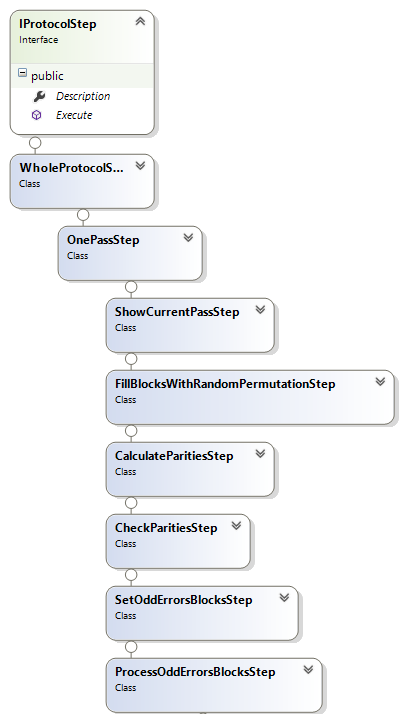
\includegraphics[width=1\linewidth]{chapter3/protocol_steps_short}
    \caption{Основные шаги, выполняемые в программе Cascade.}
    \label{fig:protocol_steps_short}
  \end{minipage}
  \hfill 
  \begin{minipage}[h]{0.4\linewidth}
    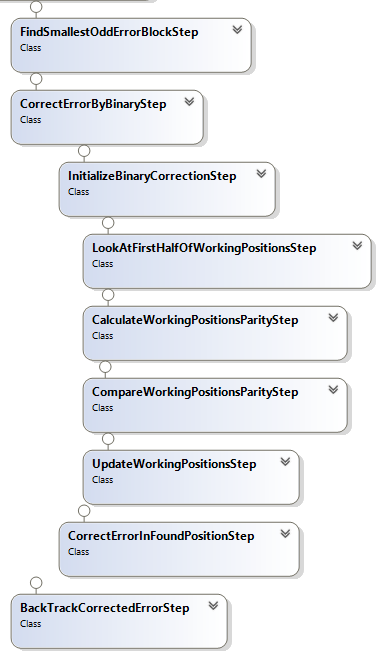
\includegraphics[width=1\linewidth]{chapter3/protocol_steps_process}
    \caption{Шаги, из которых состоит шаг ProcessOddErrorsBlocksStep.}
    \label{fig:protocol_steps_process}
  \end{minipage}
\end{center}  
\end{figure}

\FloatBarrier
\begin{figure}[h]
  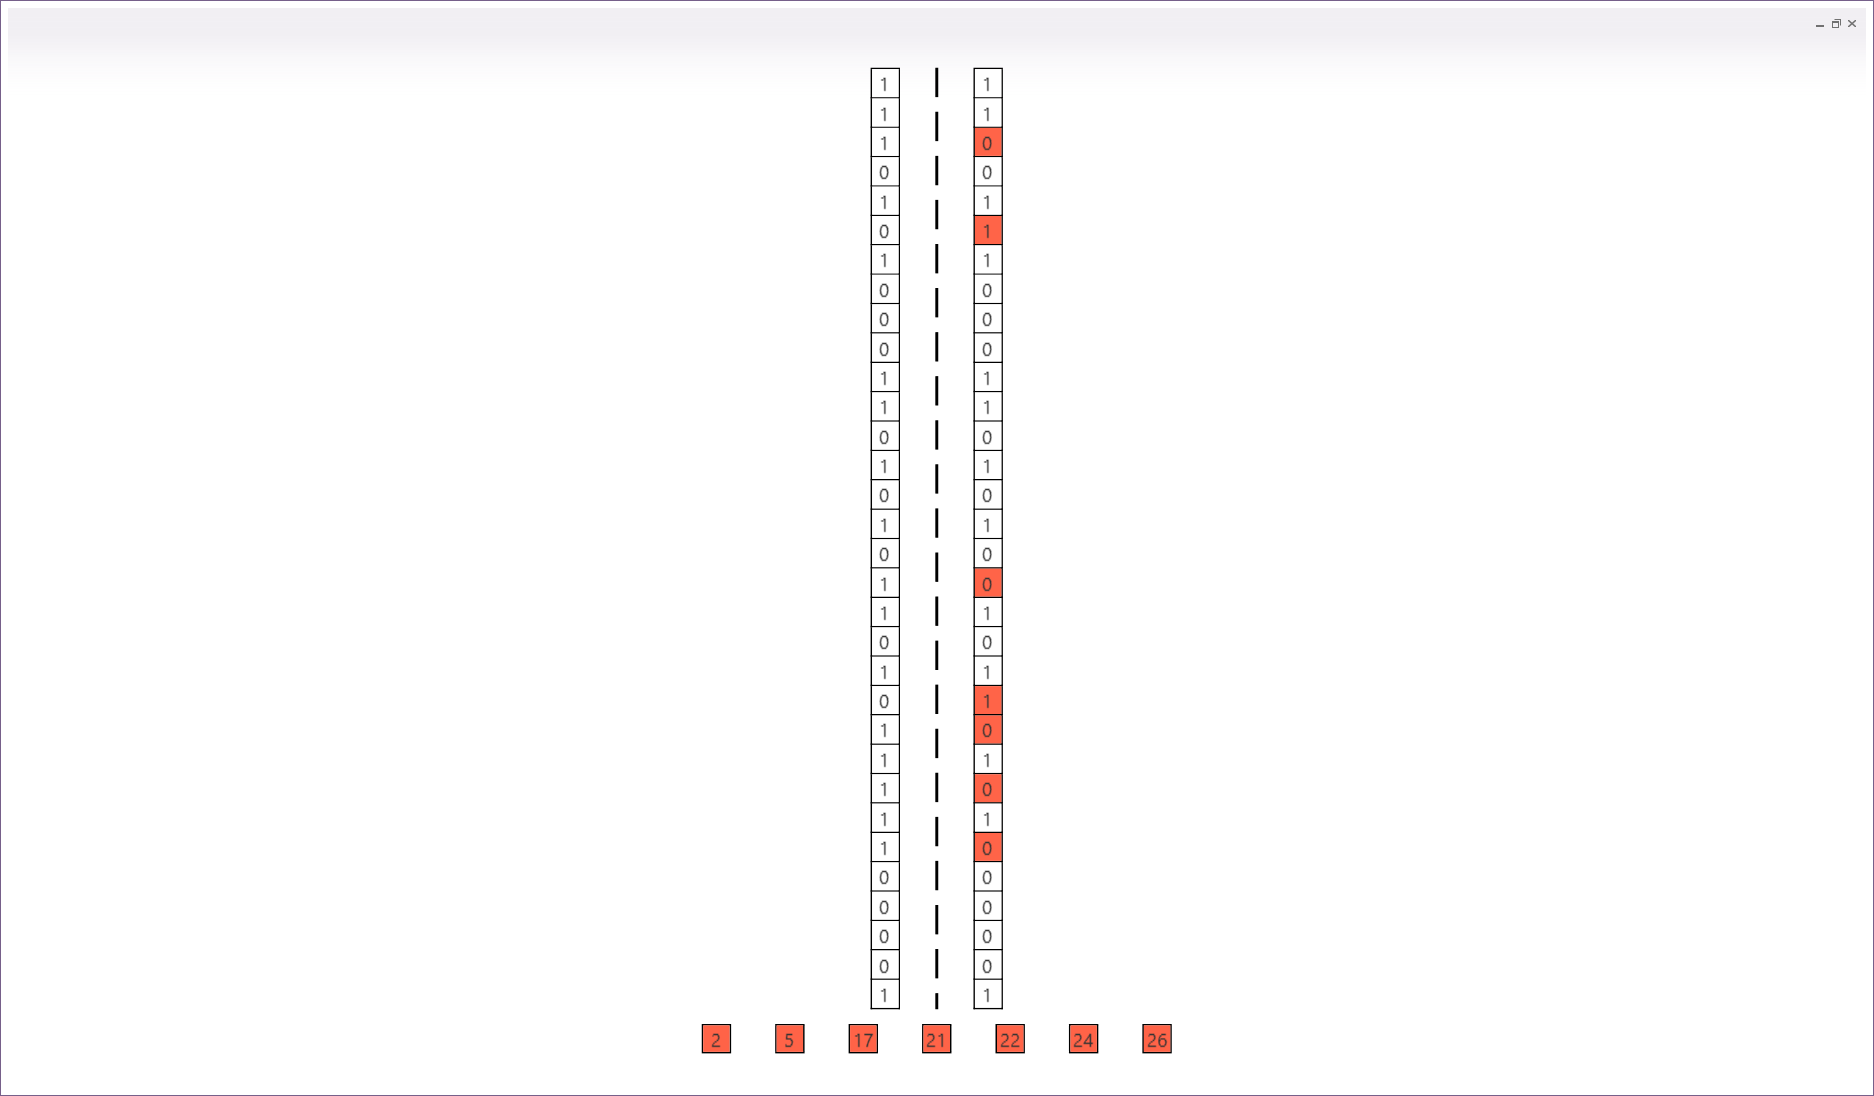
\includegraphics[width=0.9\linewidth]{chapter3/cascade_screenshots/01_start_state}
  \caption{Начальное состояние программы. Красным цветом подсвечены позиции, содержащие ошибку. Снизу указаны номера изначально ошибочных позиций для отслеживания процесса исправления.}
\end{figure}

\begin{figure}[h]
  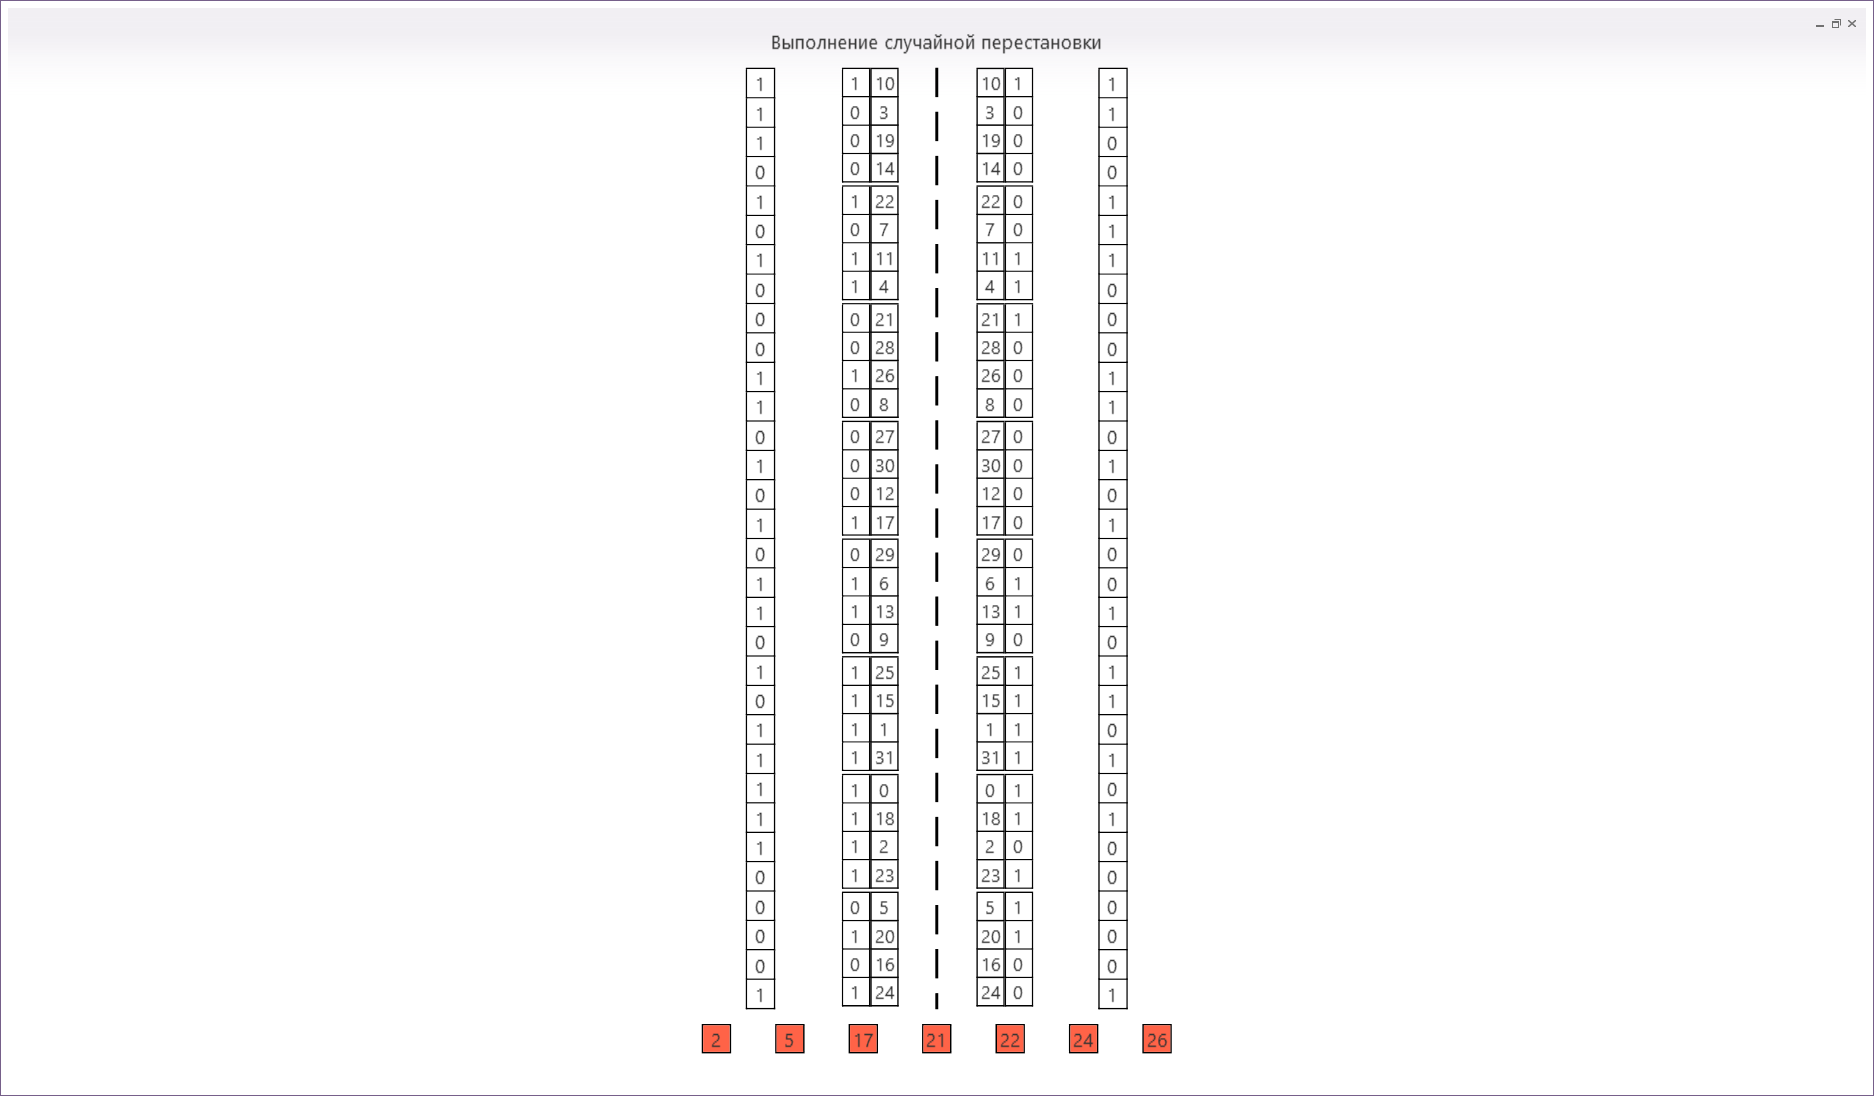
\includegraphics[width=0.9\linewidth]{chapter3/cascade_screenshots/02_fill_blocks}
  \caption{Выполнение случайной перестановки битов ключей и заполнение блоков для первого прохода.}
\end{figure}

\begin{figure}[h]
  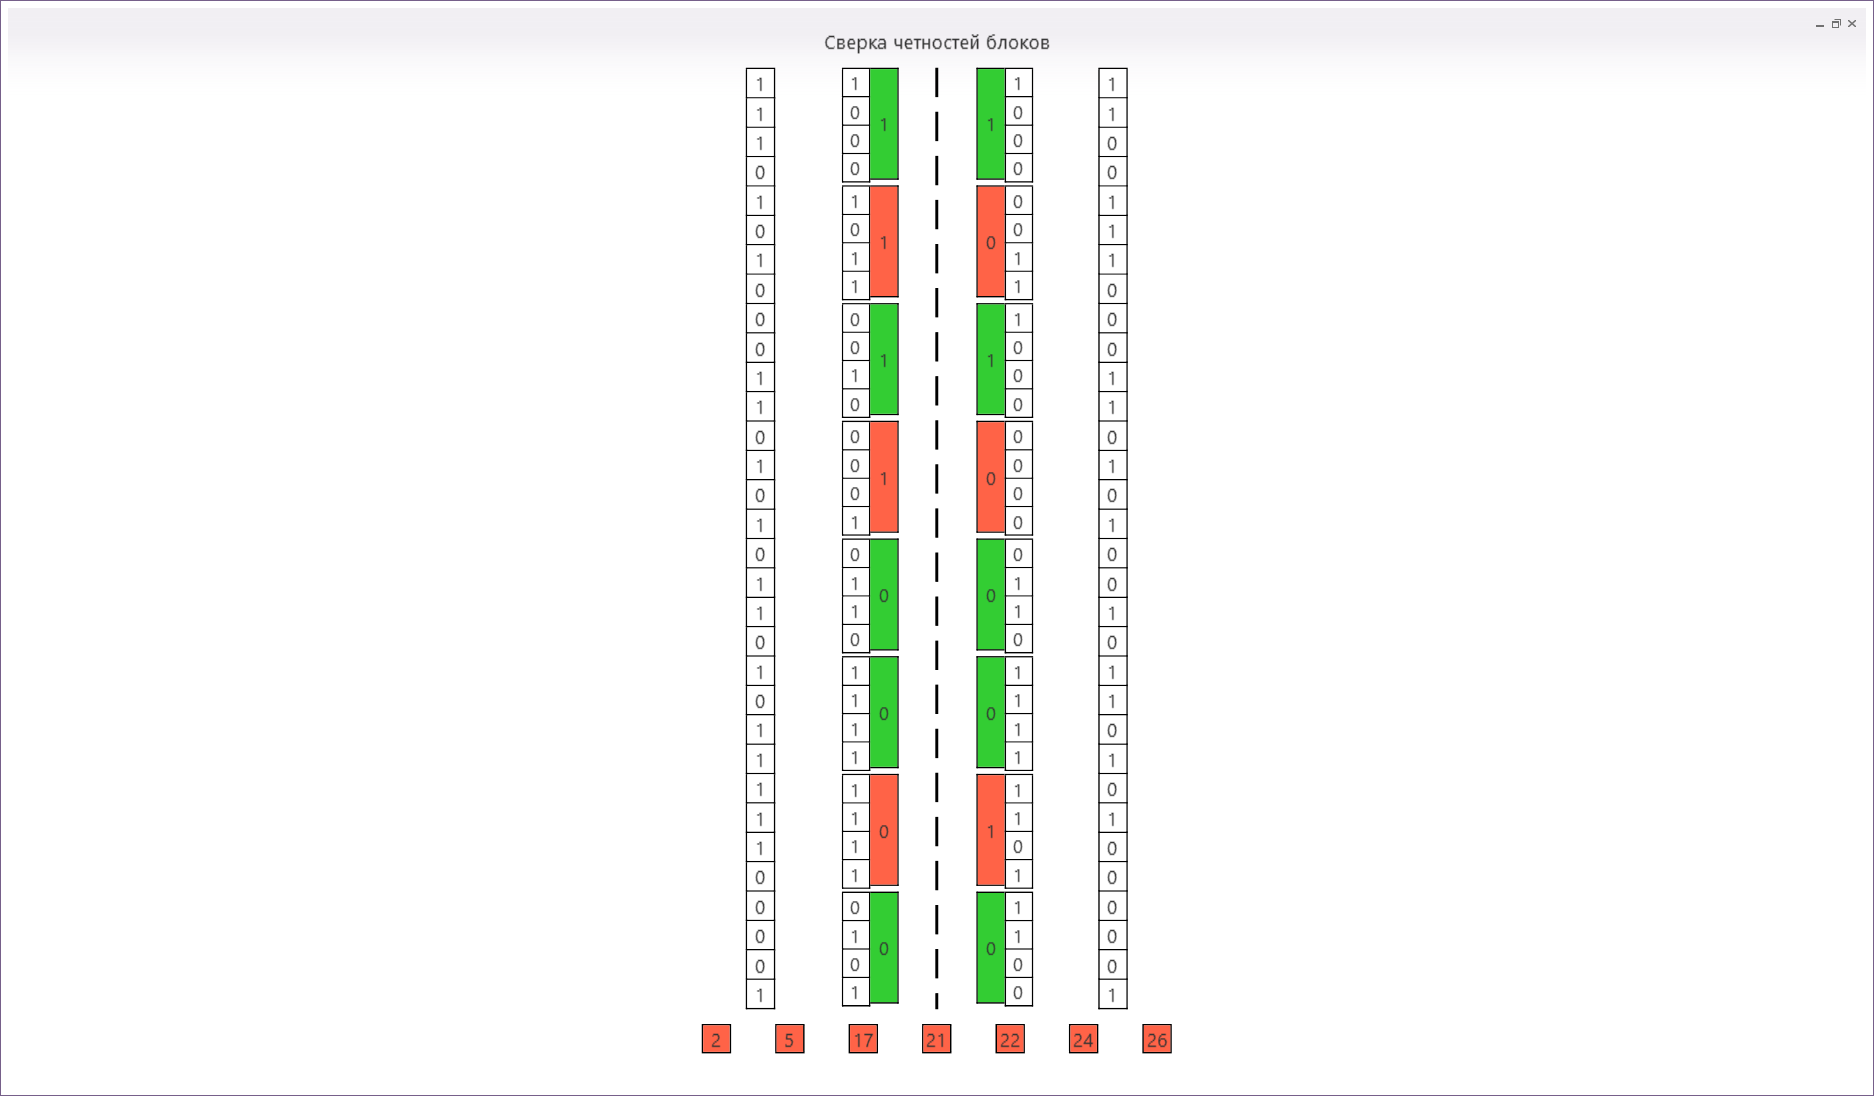
\includegraphics[width=0.9\linewidth]{chapter3/cascade_screenshots/03_check_parities}
  \caption{Сравнение четностей блоков.}
\end{figure}

\begin{figure}[h]
  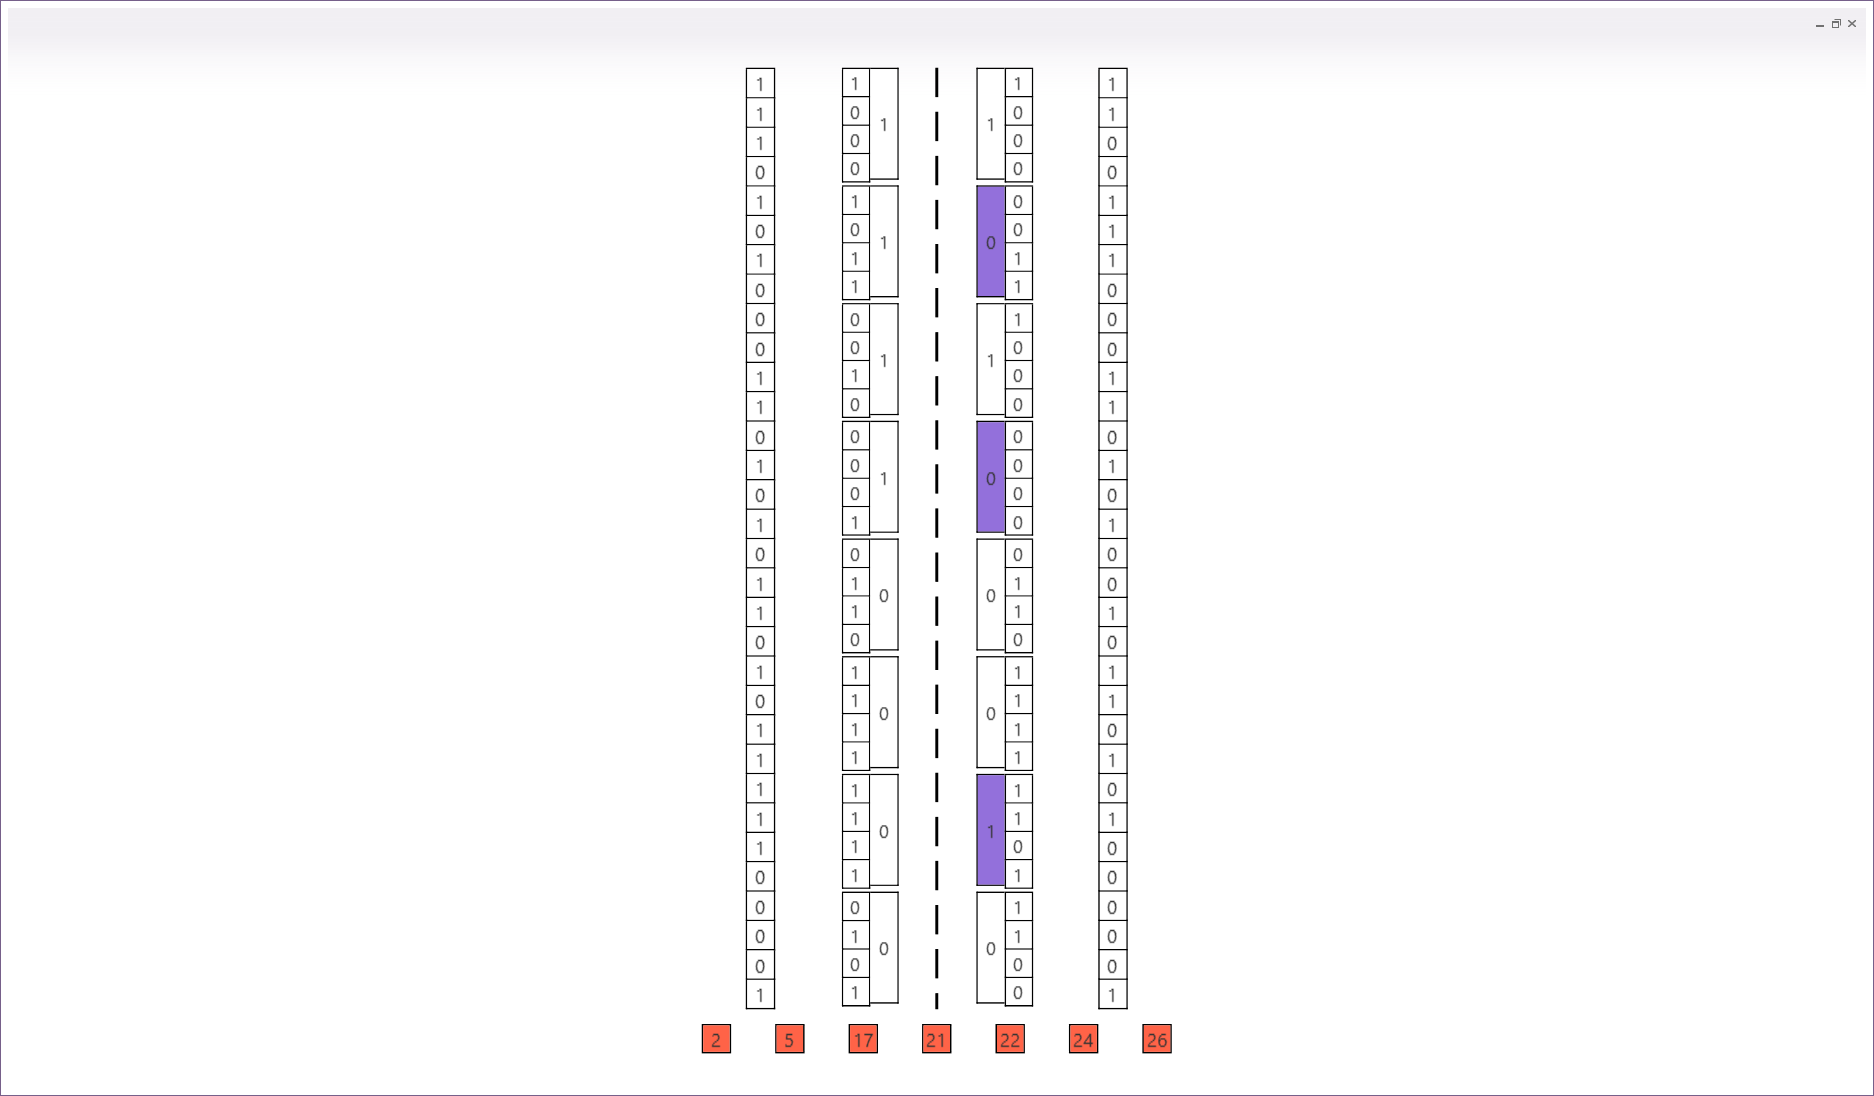
\includegraphics[width=0.9\linewidth]{chapter3/cascade_screenshots/04_set_odd_errors}
  \caption{Блоки, четности которых не совпали, формируют множество блоков с нечетным числом ошибок.}
\end{figure}

\begin{figure}[h]
  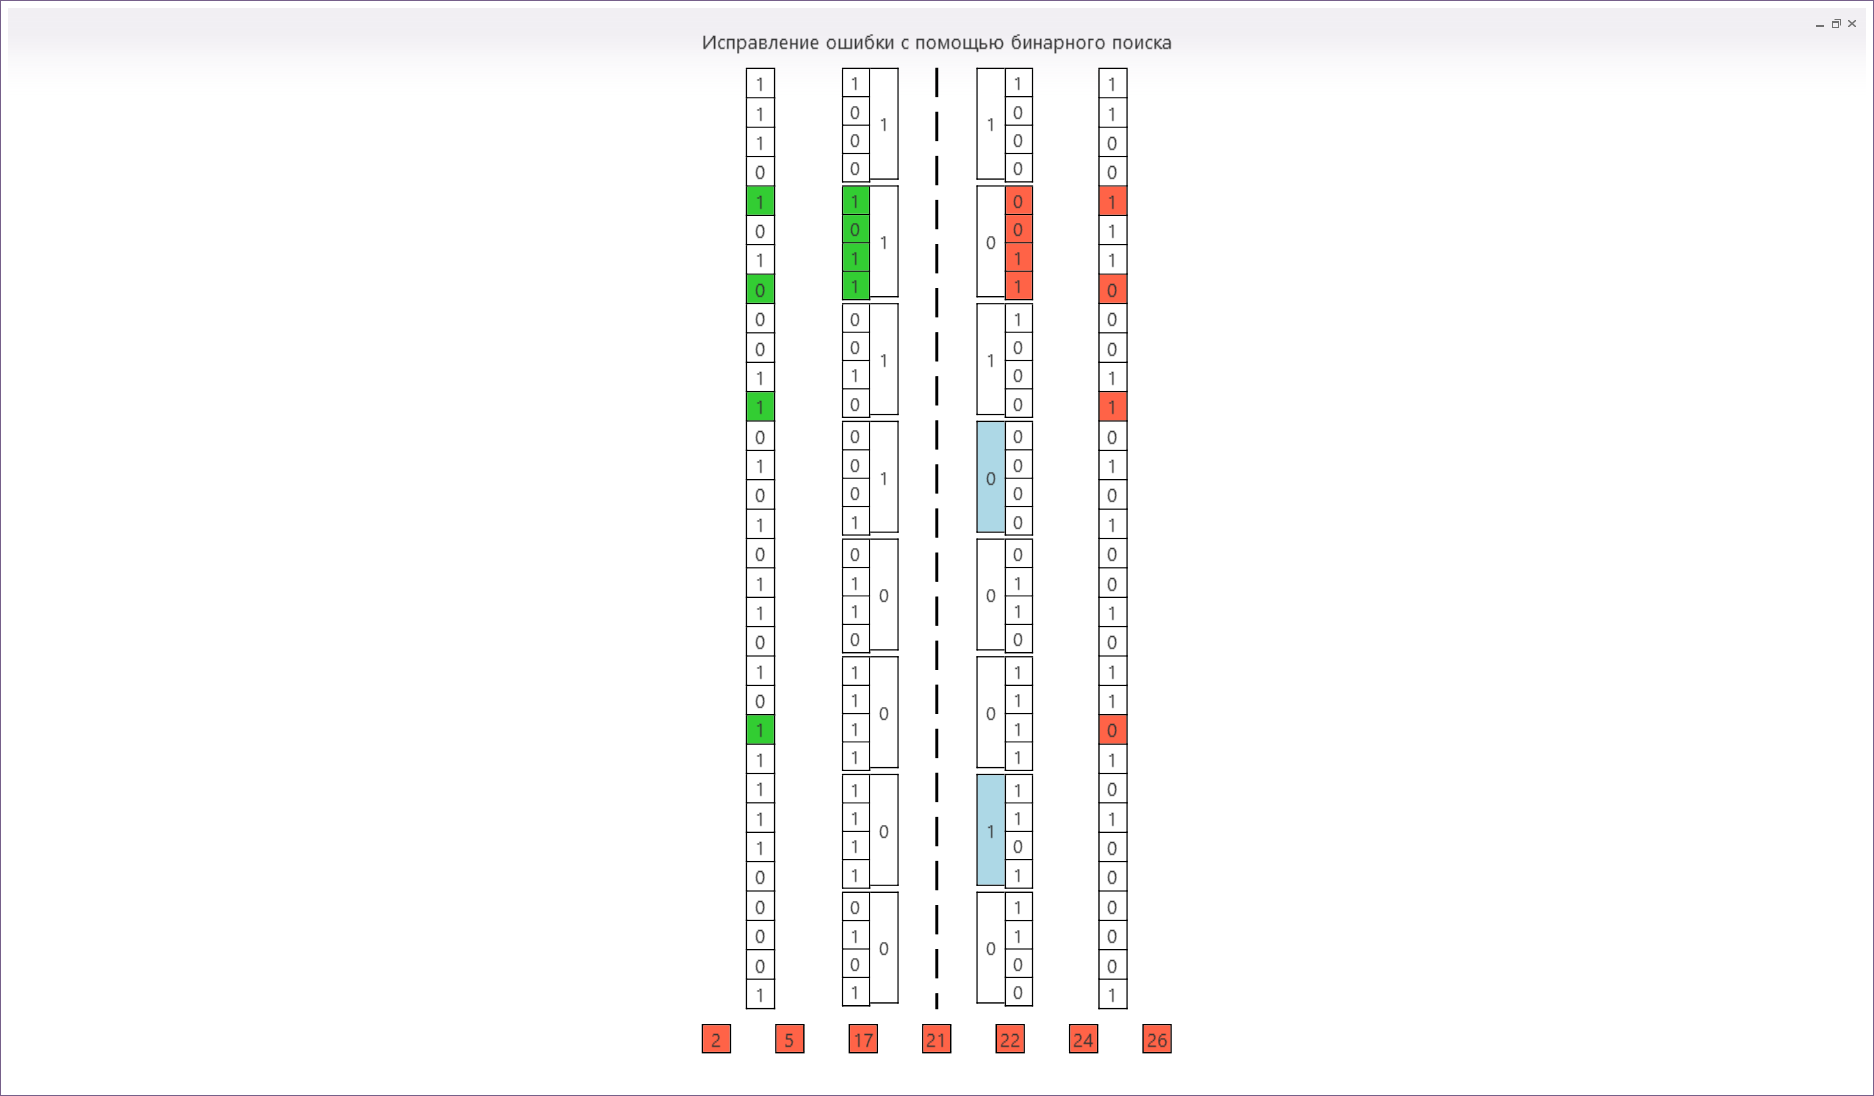
\includegraphics[width=0.9\linewidth]{chapter3/cascade_screenshots/05_binary}
  \caption{Выбирается блок из множества с нечетным числом ошибок наименьшего размера. Начинается бинарный поиск ошибки.}
\end{figure}

\begin{figure}[h]
  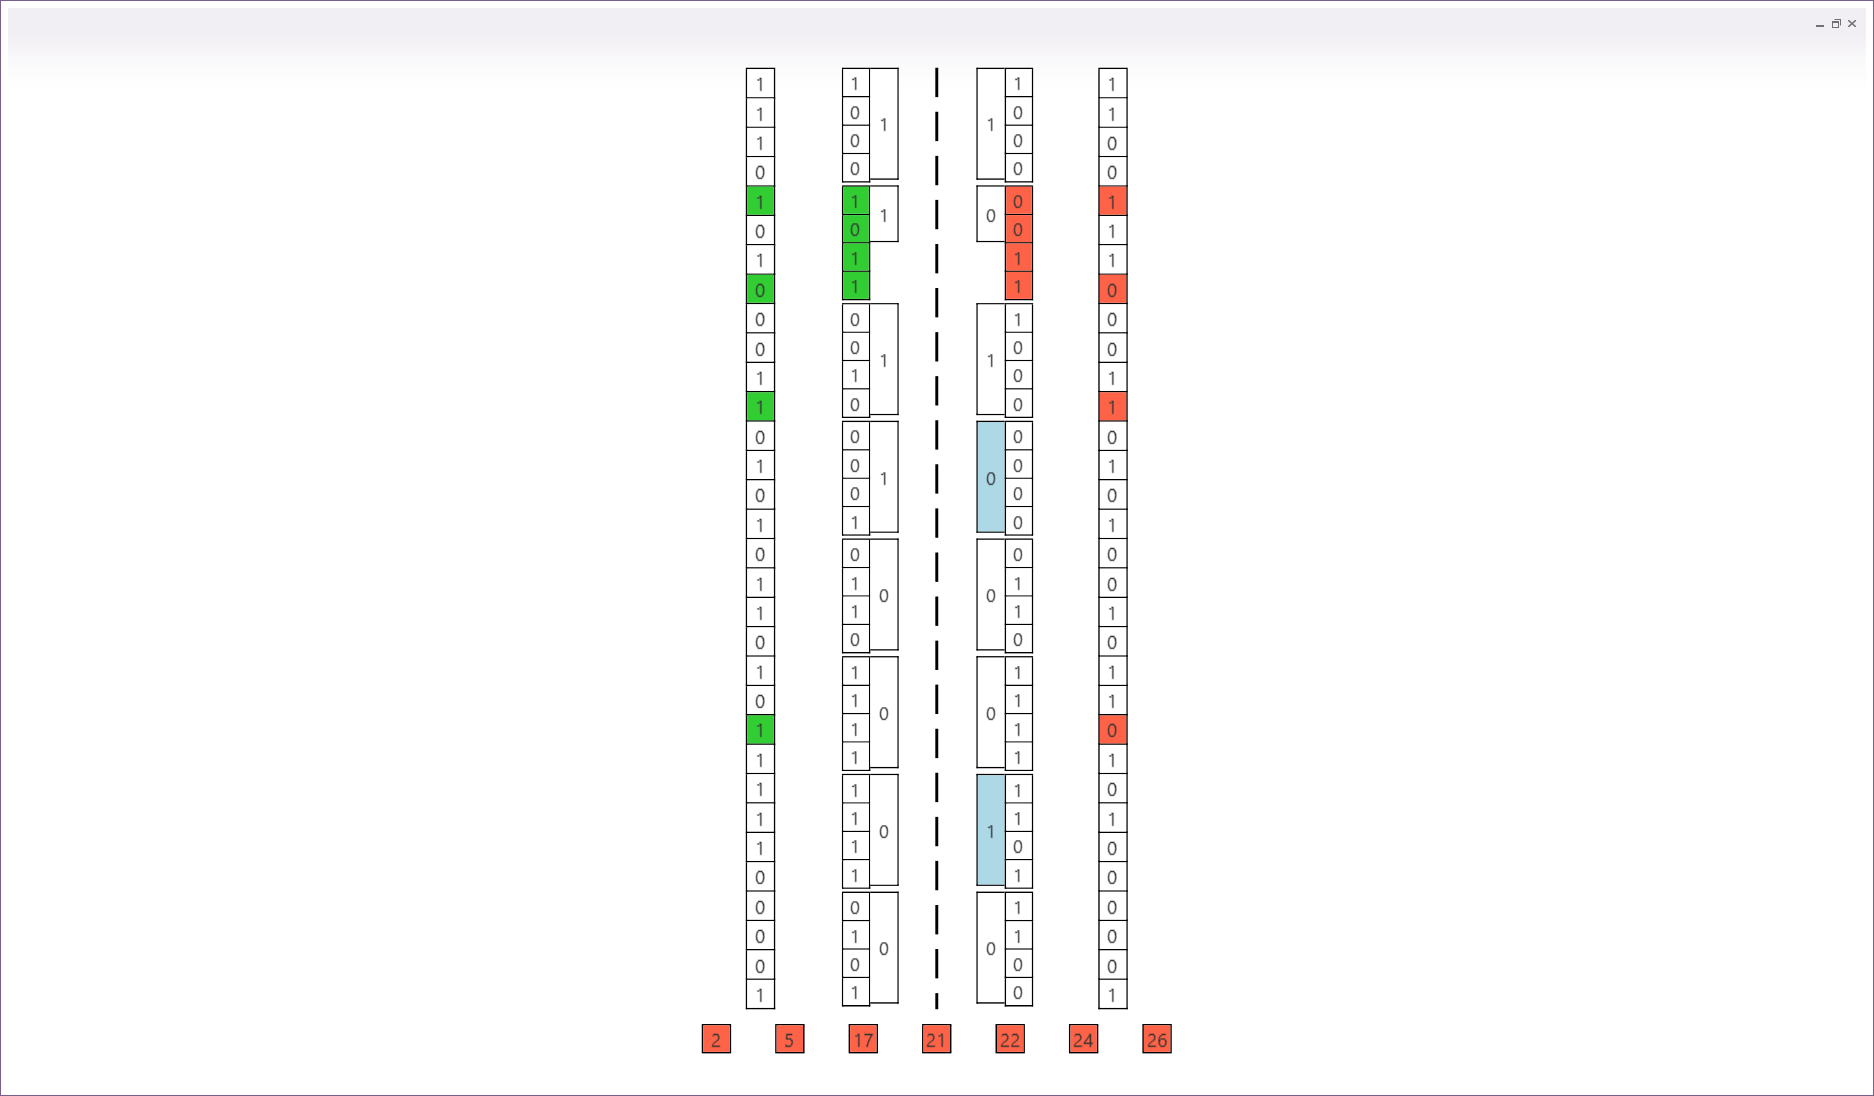
\includegraphics[width=0.9\linewidth]{chapter3/cascade_screenshots/06_binary}
  \caption{Сравнение четности первой половины блока. В данном случае совпадения нет, значит, ошибка находится среди бит первой половины.}
\end{figure}

\begin{figure}[h]
  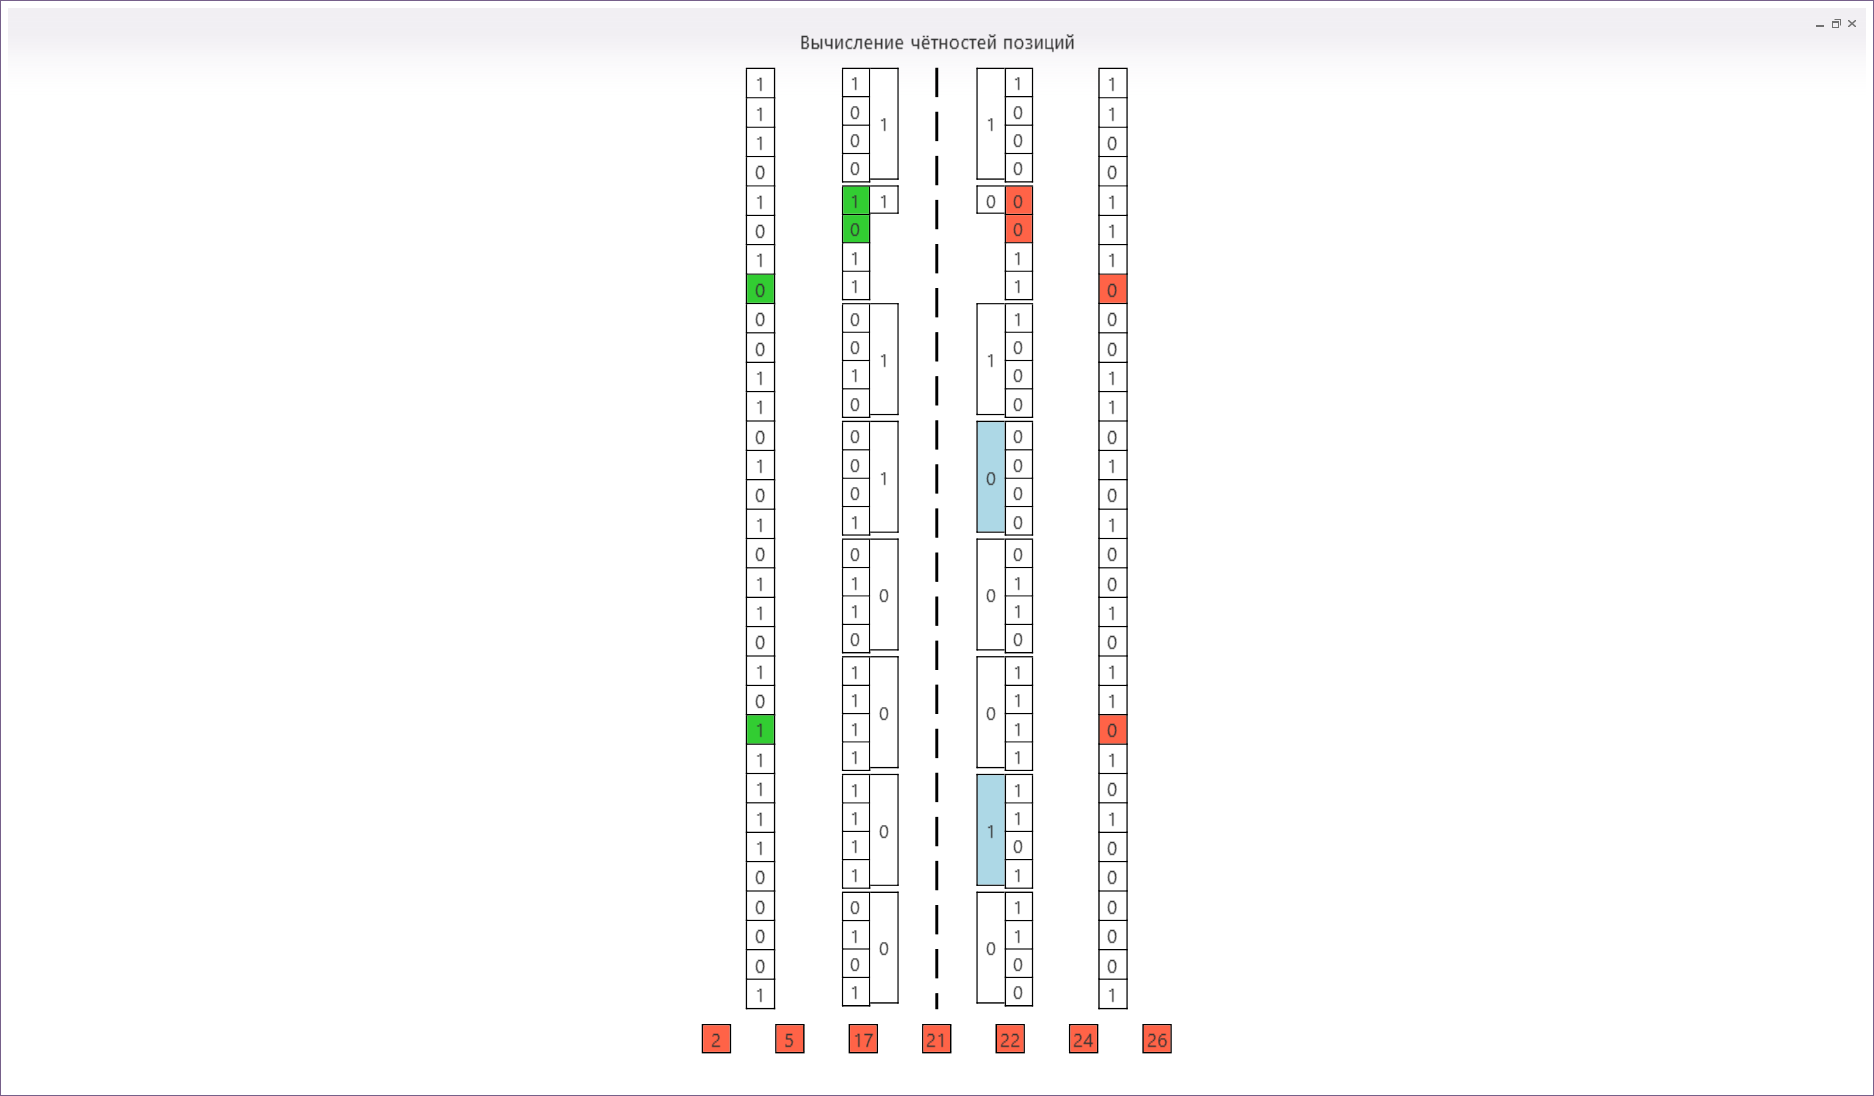
\includegraphics[width=0.9\linewidth]{chapter3/cascade_screenshots/07_binary}
  \caption{Последнее сравнение четностей, размер половины блока достиг одного бита.}
\end{figure}

\begin{figure}[h]
  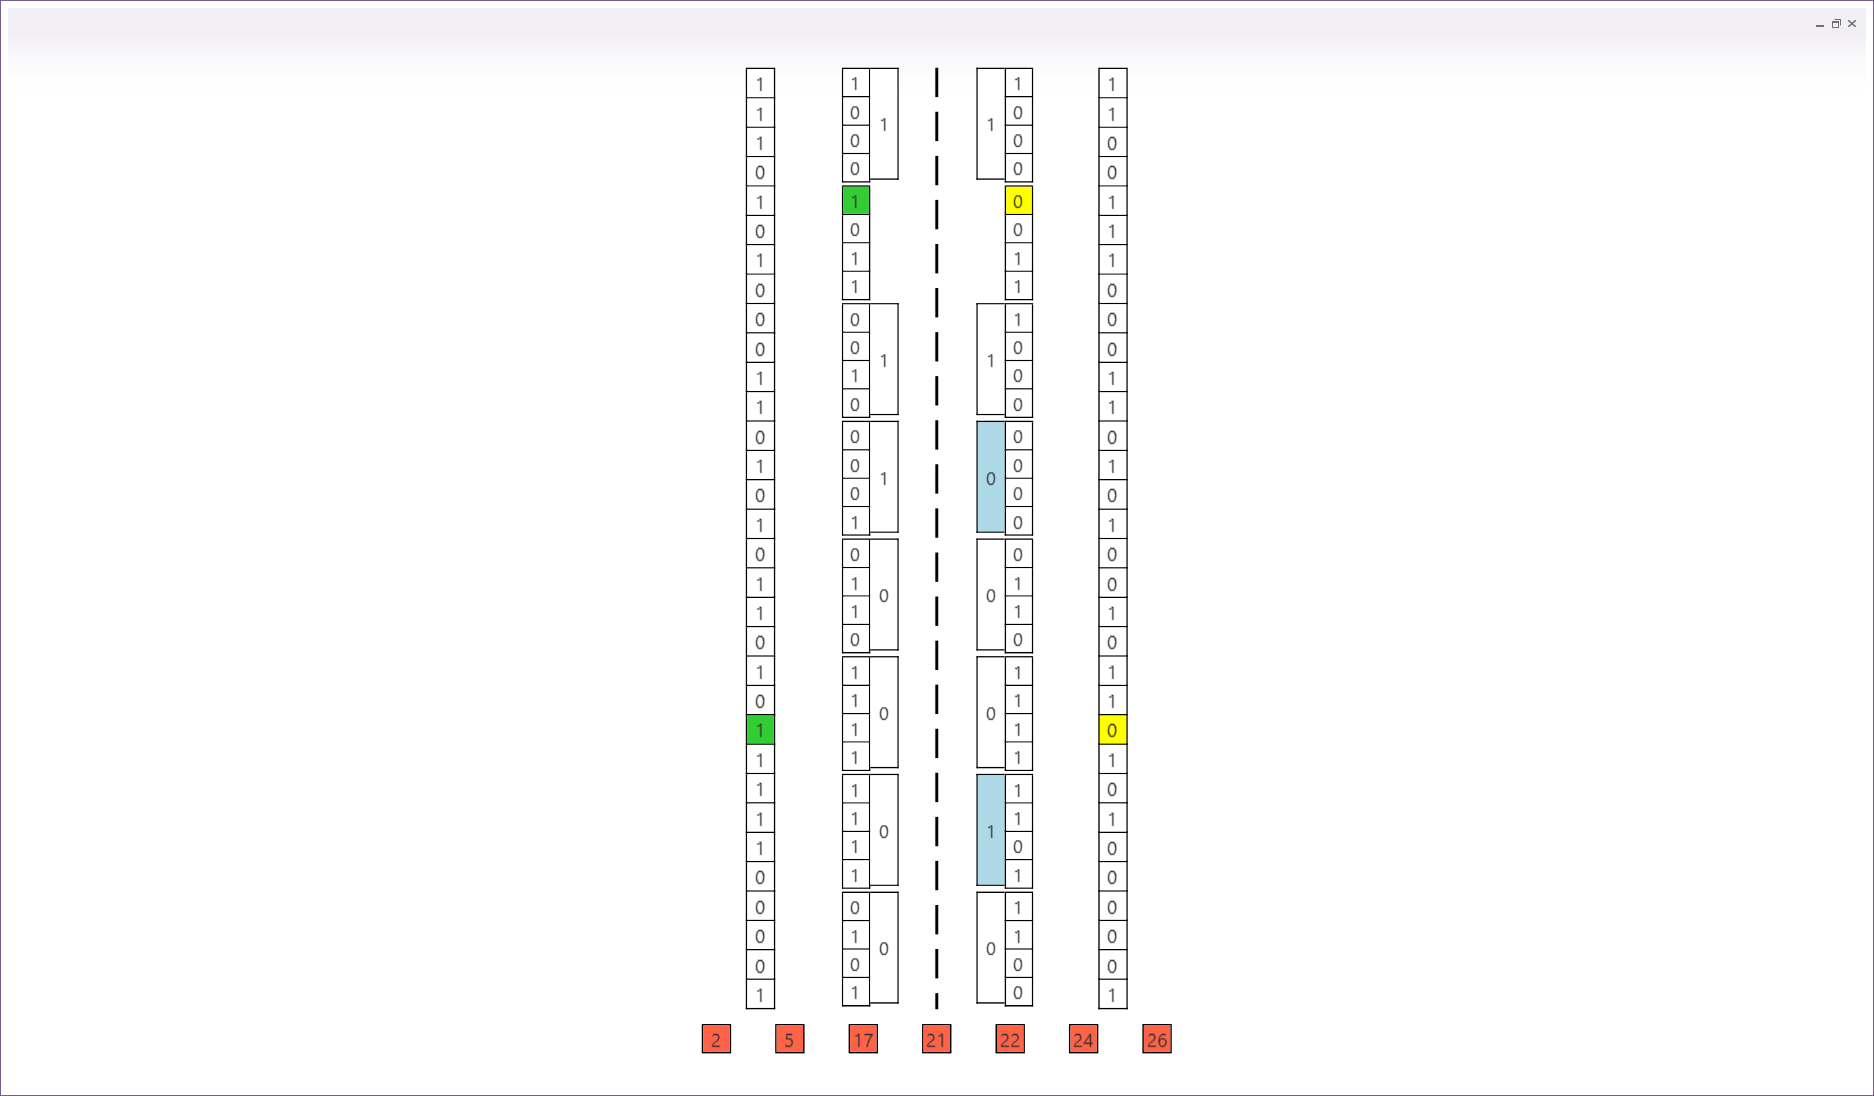
\includegraphics[width=0.9\linewidth]{chapter3/cascade_screenshots/08_found_error}
  \caption{Ошибка найдена.}
\end{figure}

\begin{figure}[h]
  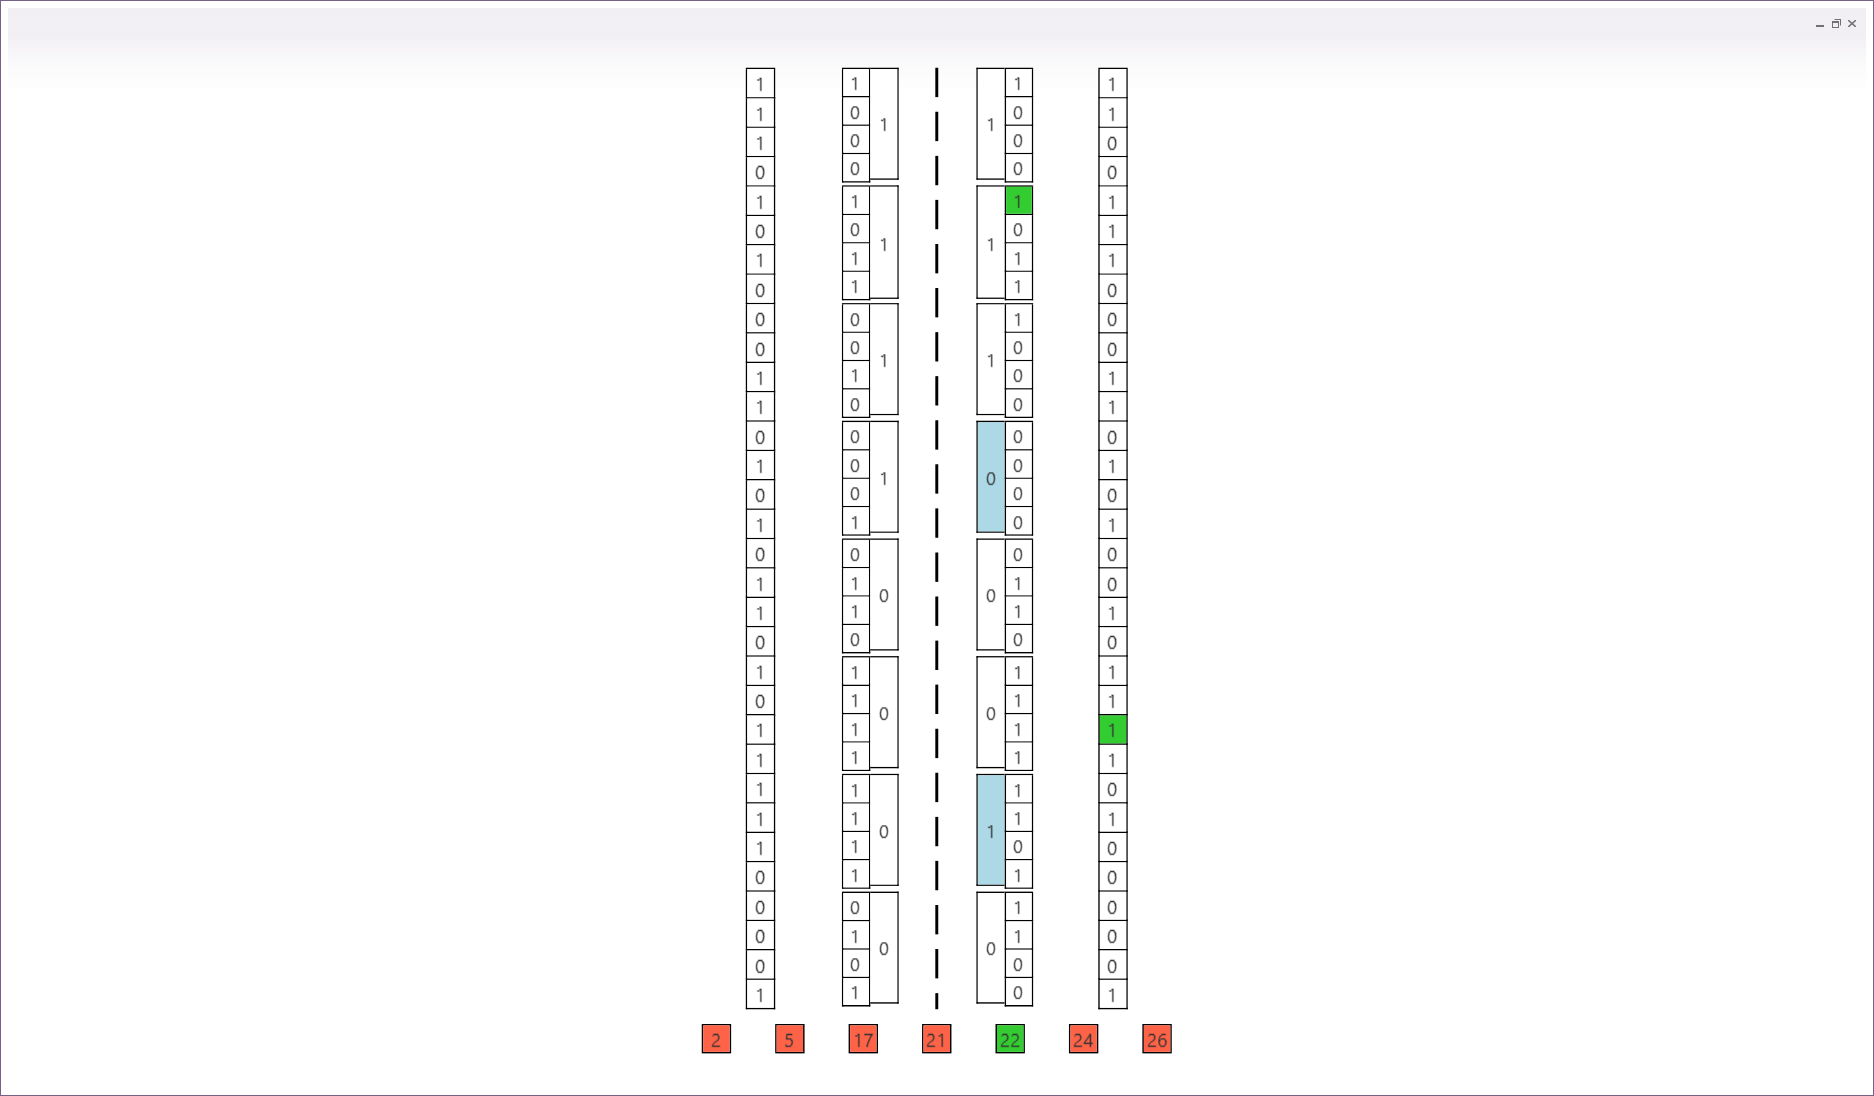
\includegraphics[width=0.9\linewidth]{chapter3/cascade_screenshots/09_error_corrected}
  \caption{Ошибка исправлена. Процесс будет повторен с оставшимися блоками с нечетным числом ошибок.}
\end{figure}

\begin{figure}[h]
  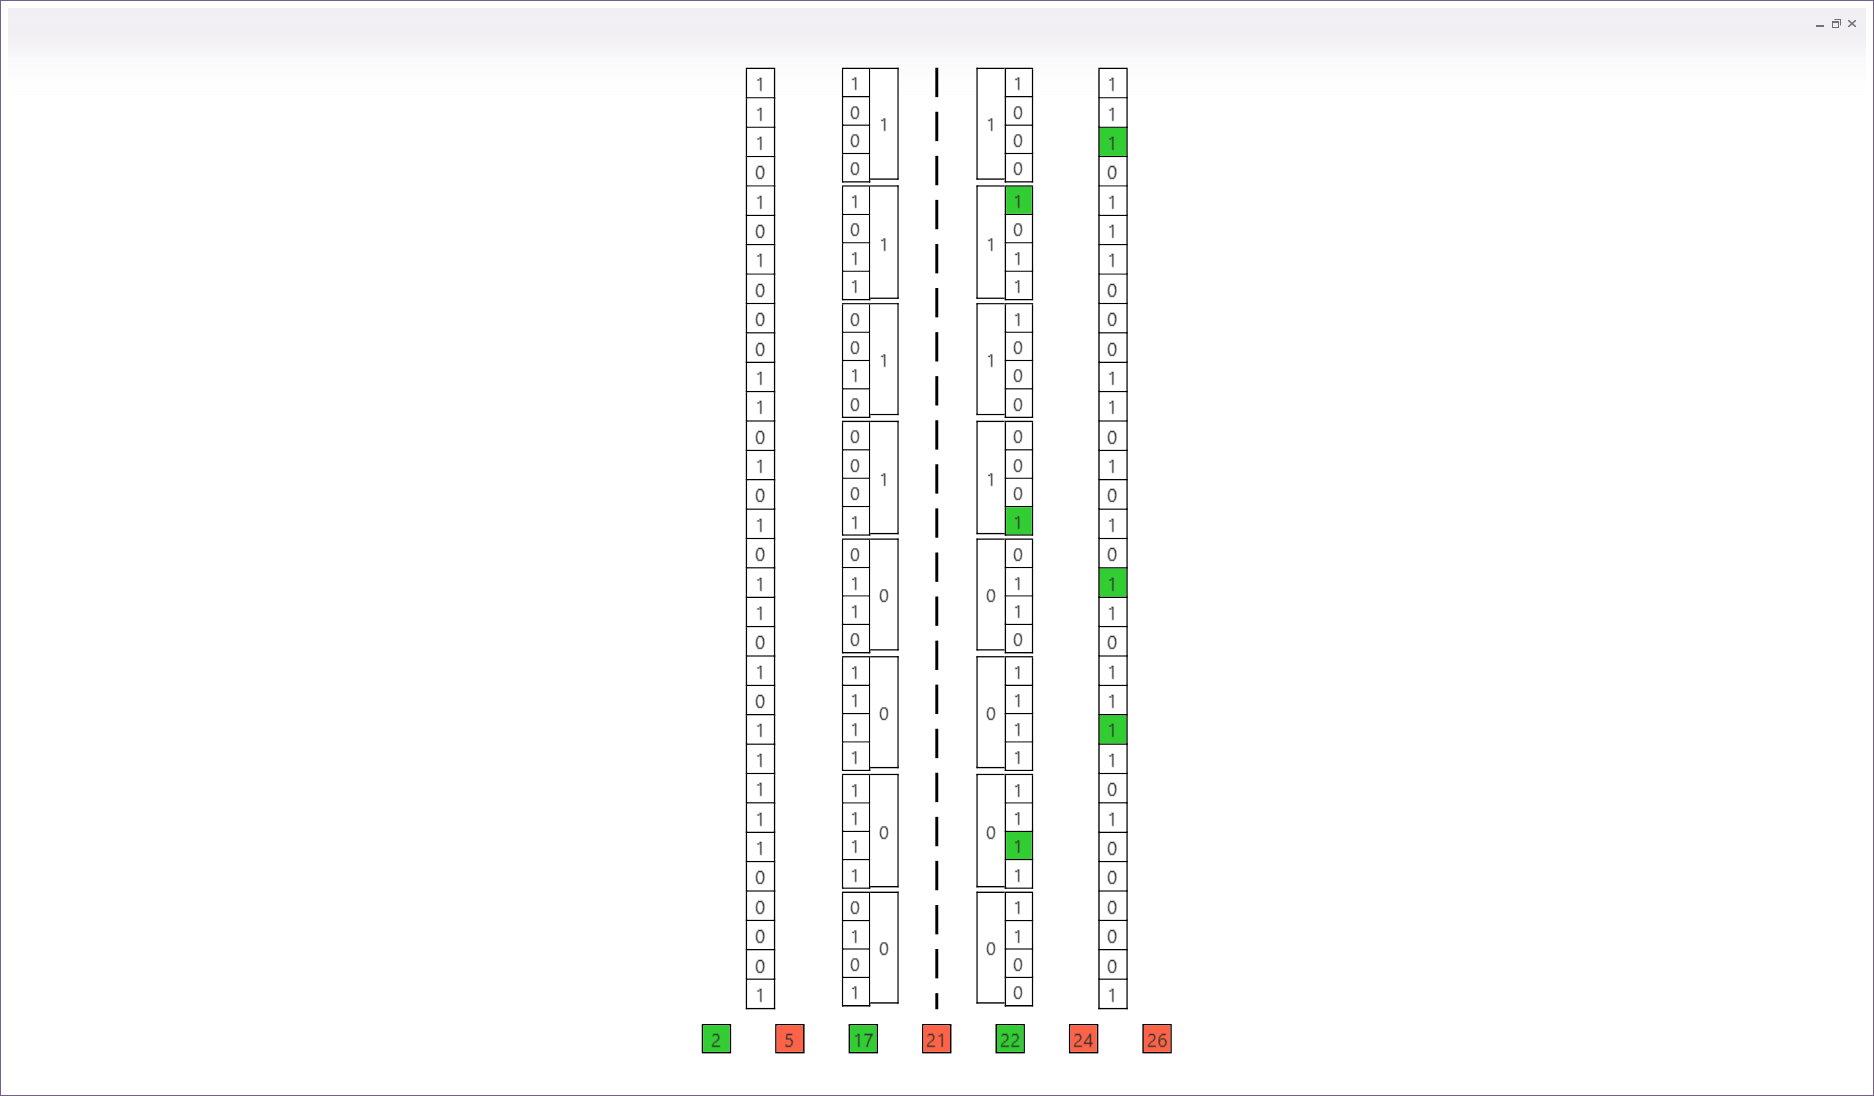
\includegraphics[width=0.9\linewidth]{chapter3/cascade_screenshots/10_pass_complete}
  \caption{Исправлены все ошибки на текущем проходе.}
\end{figure}

\begin{figure}[h]
  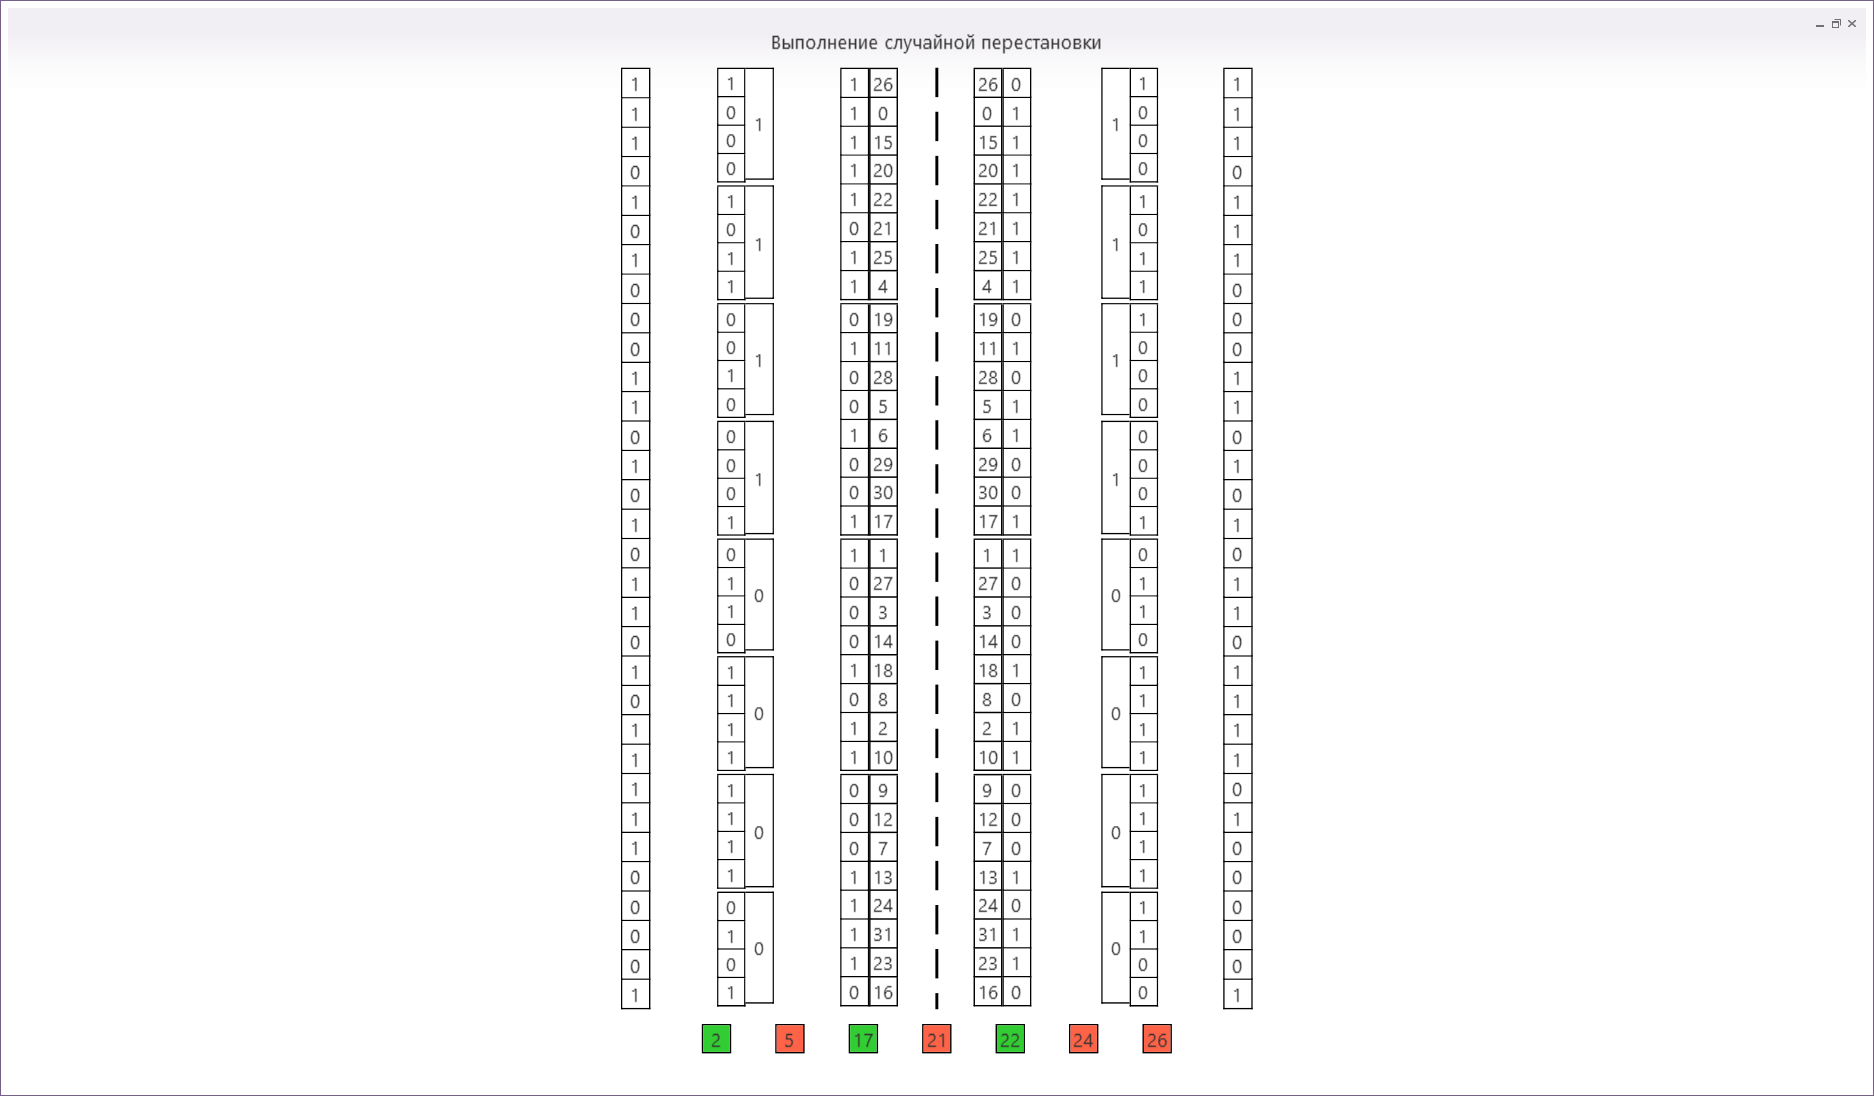
\includegraphics[width=0.9\linewidth]{chapter3/cascade_screenshots/11_fill_blocks}
  \caption{Начало следующего прохода. Размер блока увеличивается вдвое. Выполняется новая случайная перестановка битов ключей.}
\end{figure}

\begin{figure}[h]
  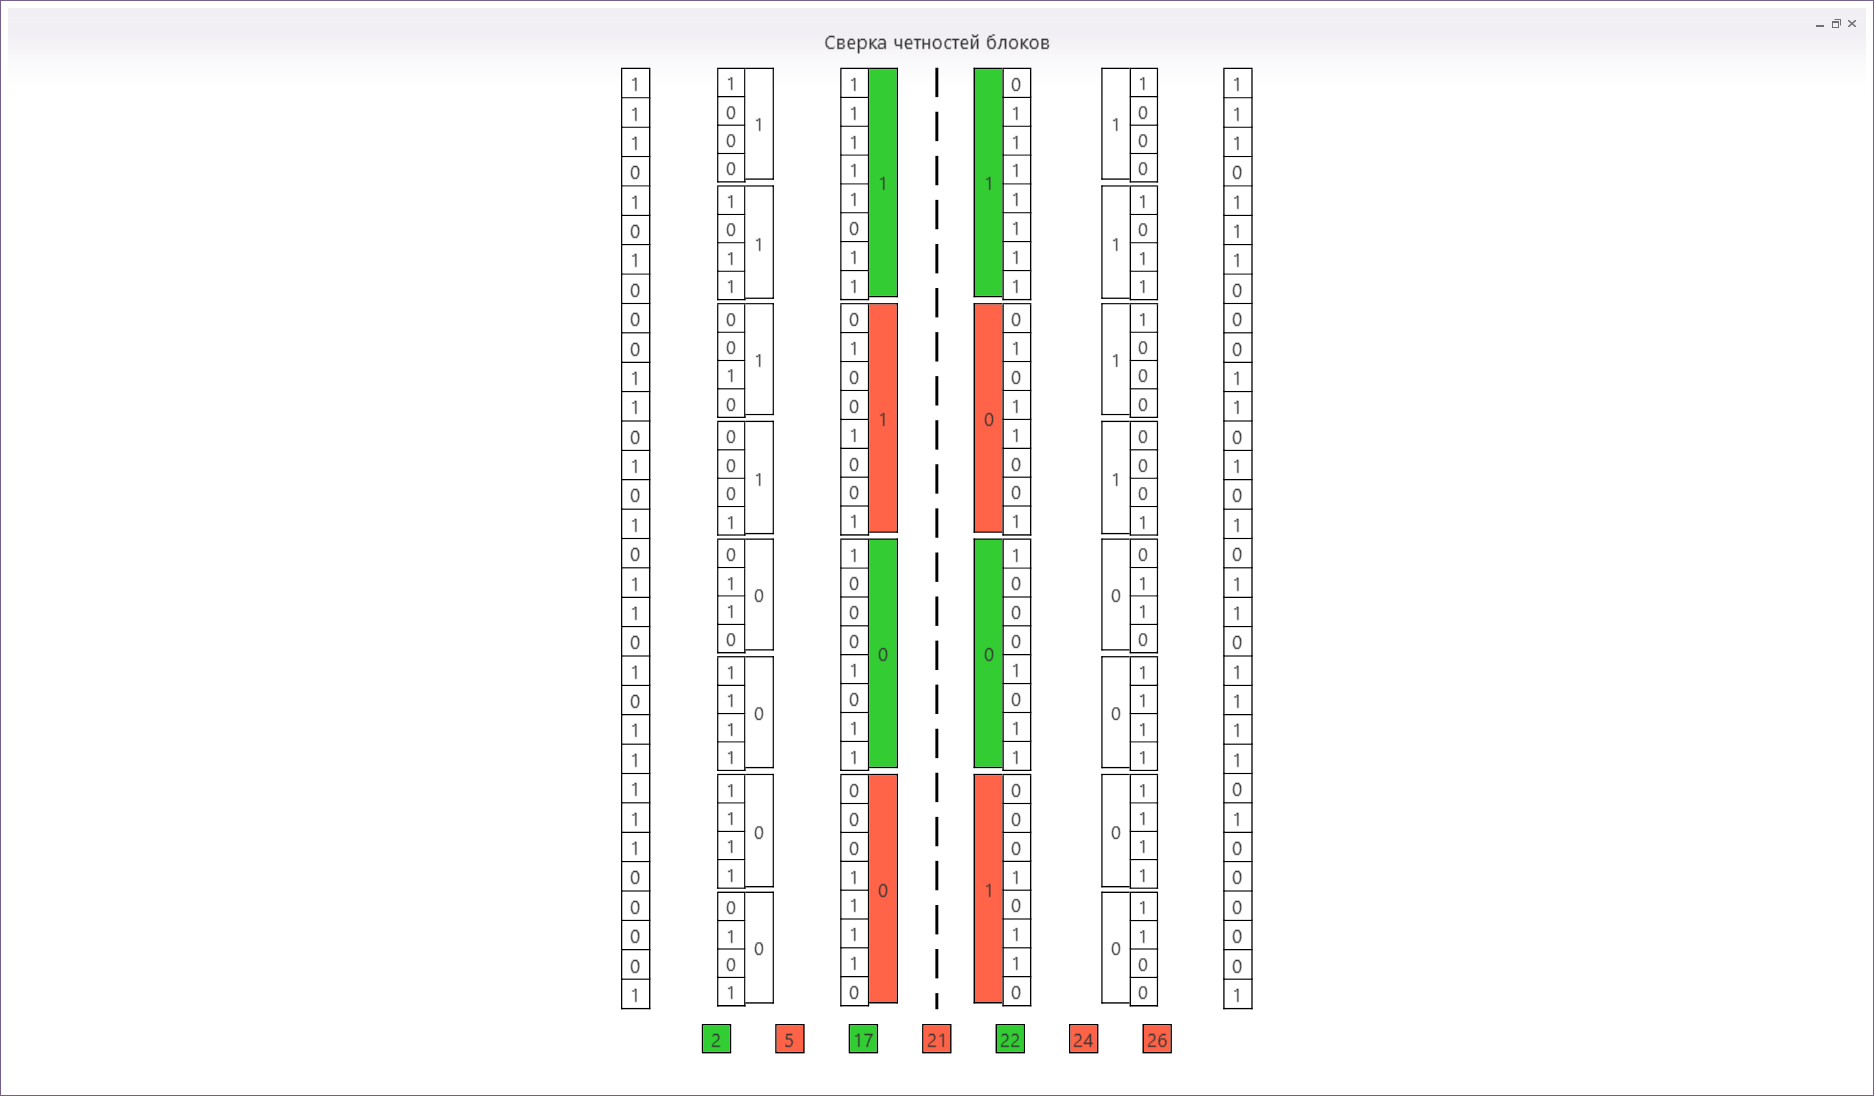
\includegraphics[width=0.9\linewidth]{chapter3/cascade_screenshots/12_check_parities}
  \caption{Сверка четностей блоков текущего прохода.}
\end{figure}

\begin{figure}[h]
  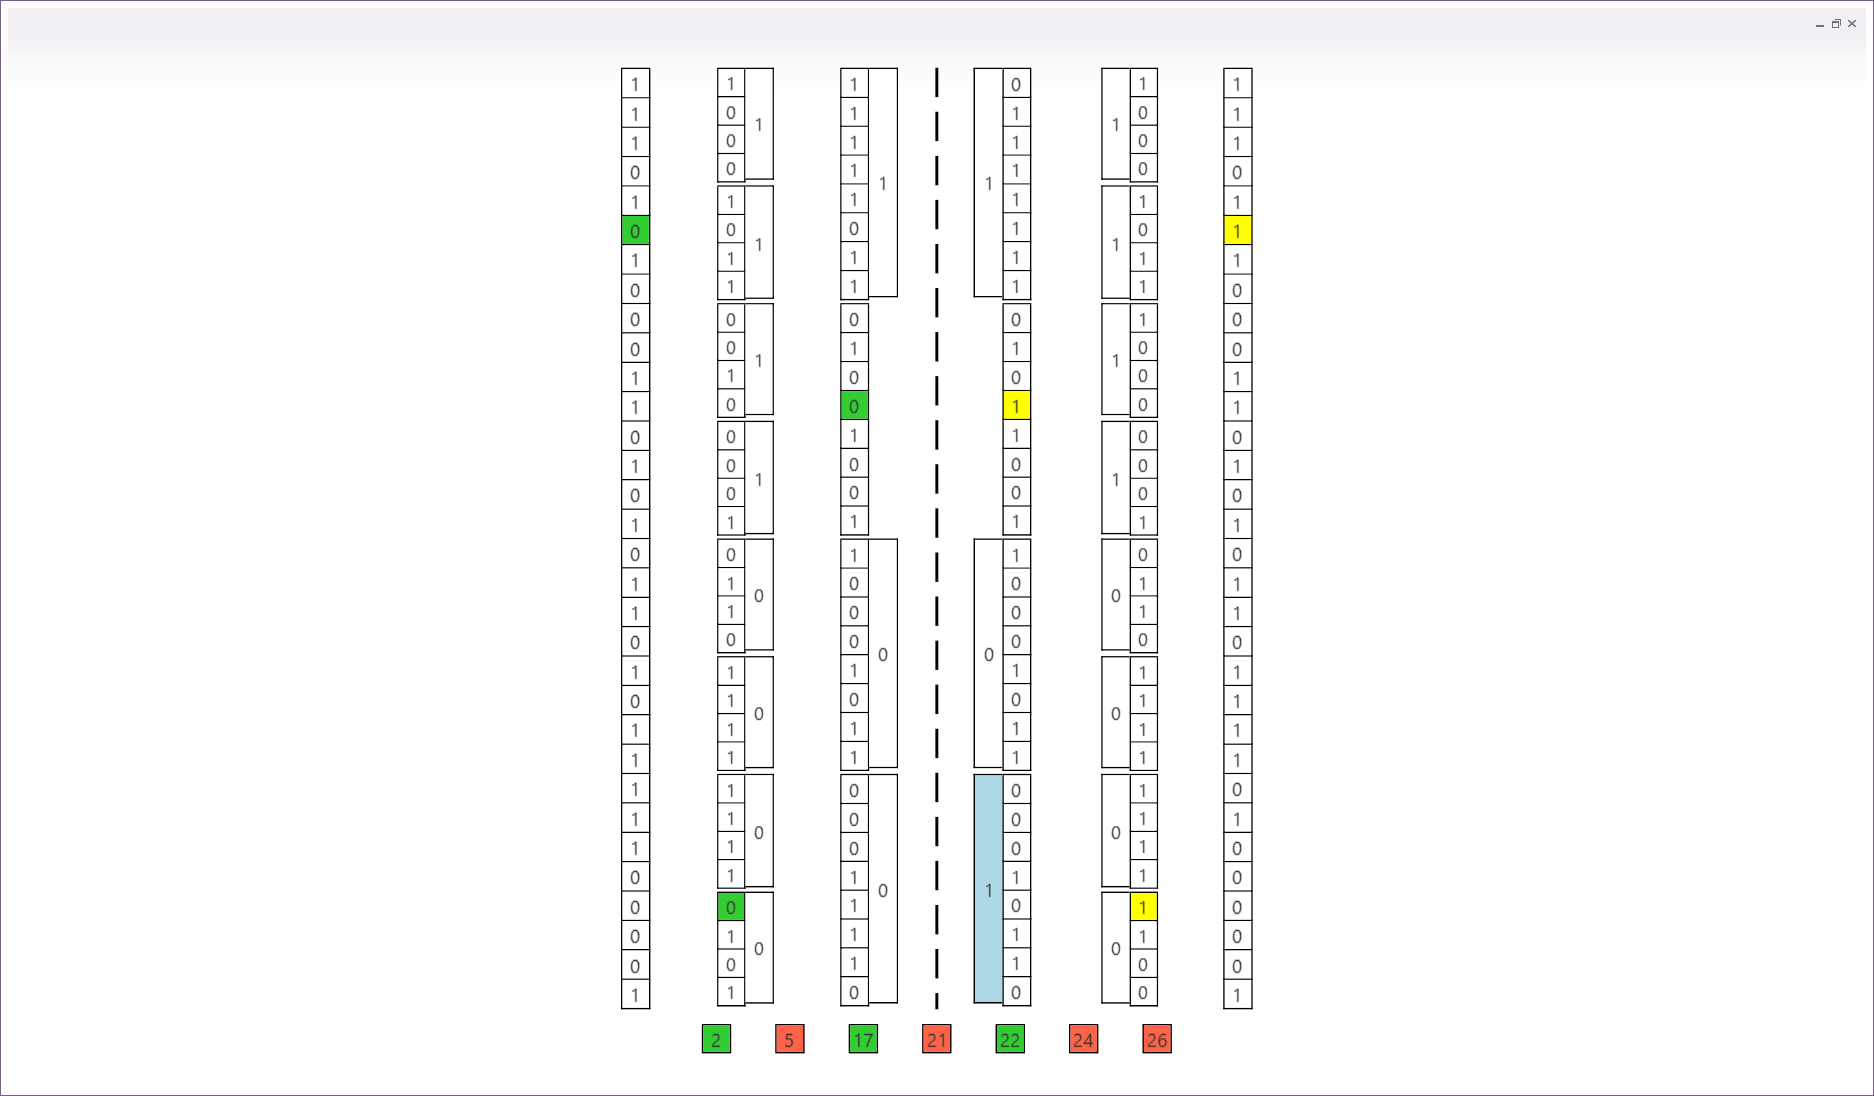
\includegraphics[width=0.9\linewidth]{chapter3/cascade_screenshots/13_error_found}
  \caption{Двоичным поиском найдена ошибочная позиция в одном из блоков.}
\end{figure}

\begin{figure}[h]
  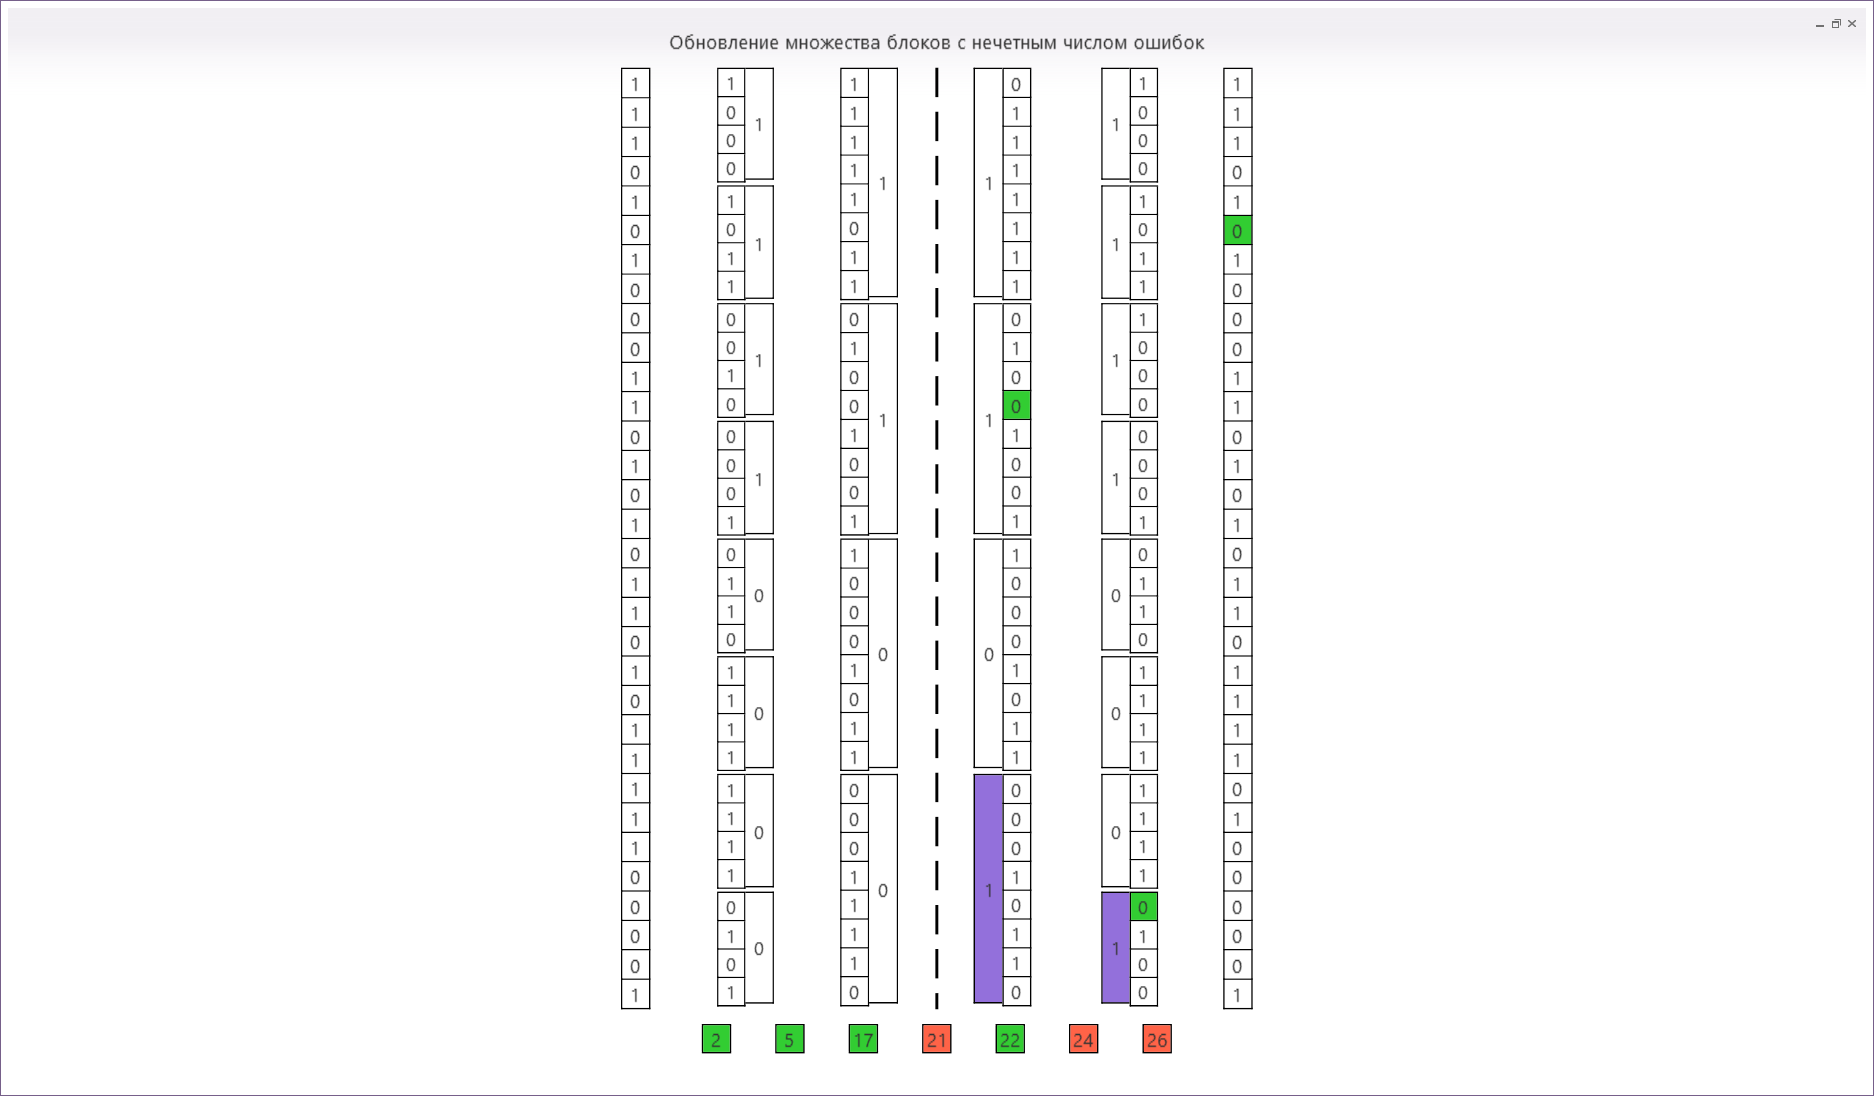
\includegraphics[width=0.9\linewidth]{chapter3/cascade_screenshots/14_error_backtrace}
  \caption{Все блоки (в этом примере нижний из первого прохода), которые содержат исправленную позицию, попадают в множество блоков с нечетным числом ошибок, если еще не входили в него.}
\end{figure}

\begin{figure}[h]
  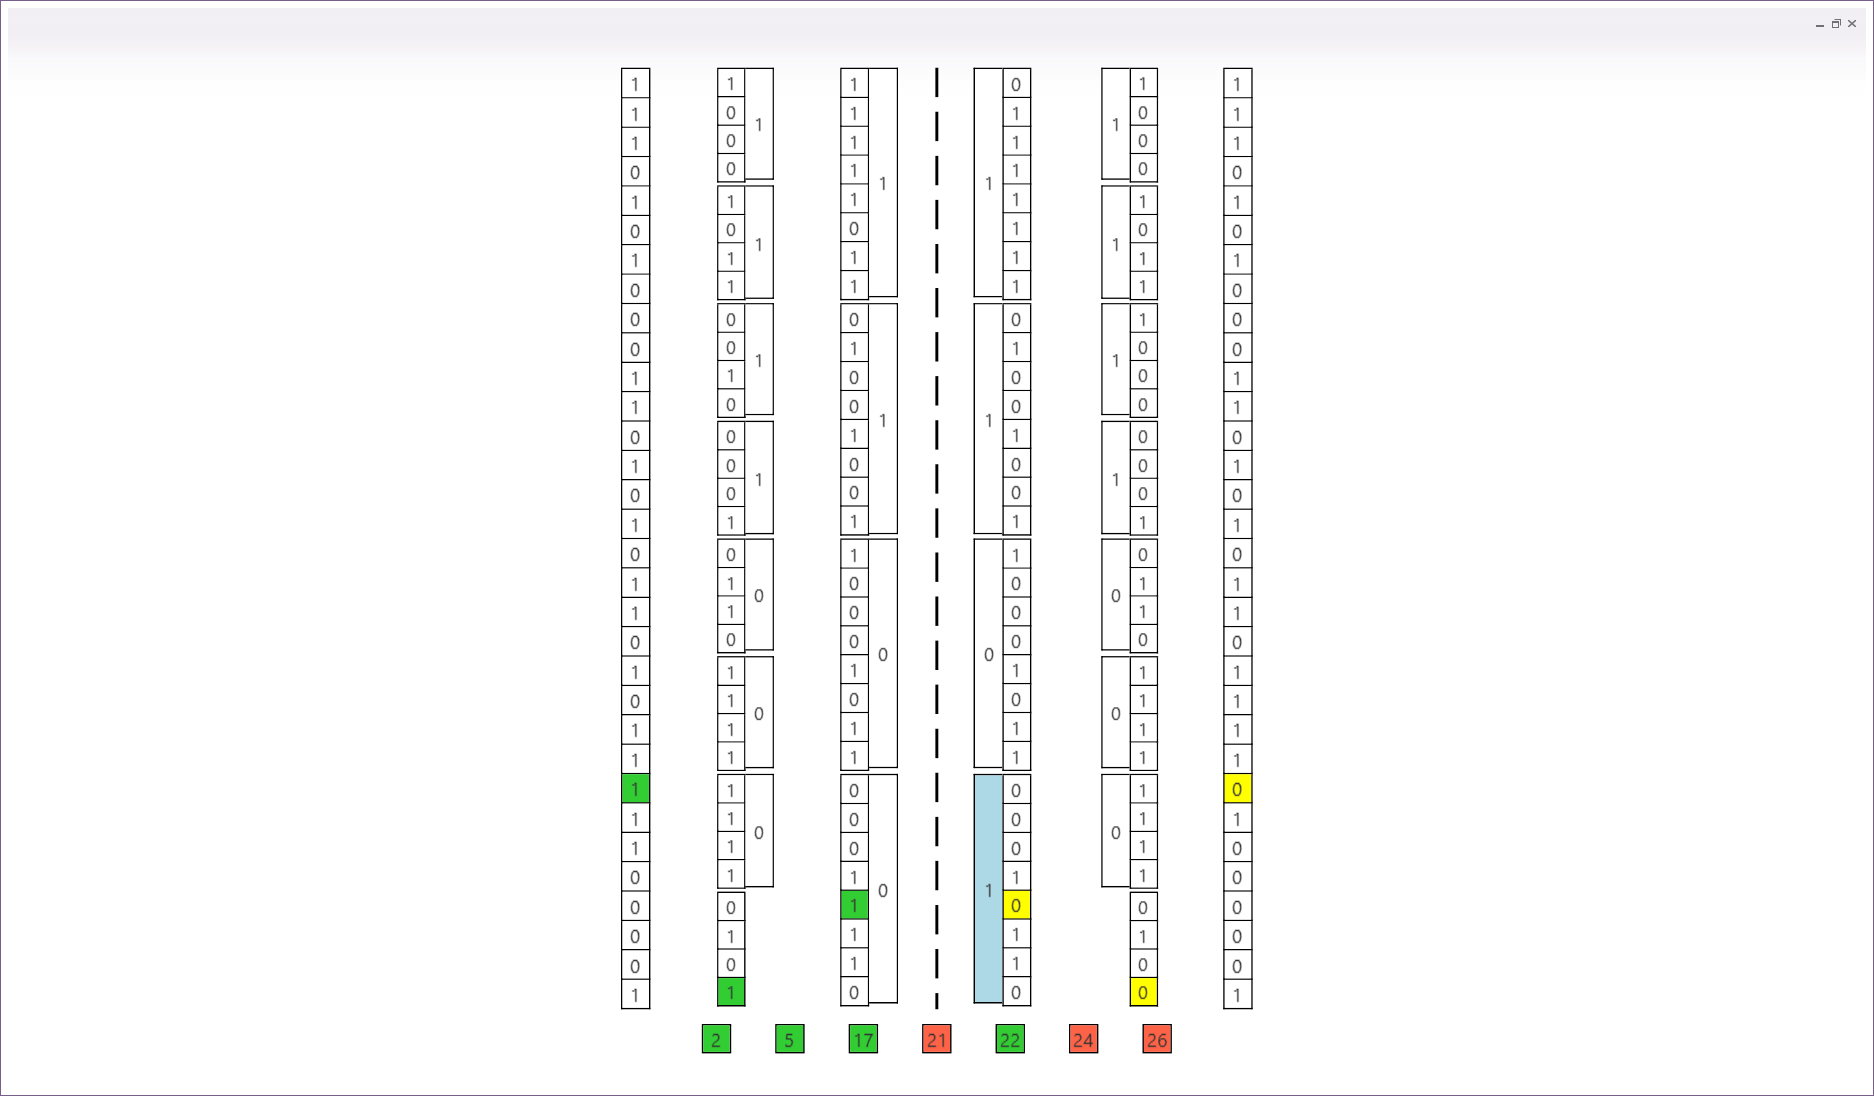
\includegraphics[width=0.9\linewidth]{chapter3/cascade_screenshots/15_error_found}
  \caption{В блоке наименьшего размера снова находится ошибочная позиция.}
\end{figure}

\begin{figure}[h]
  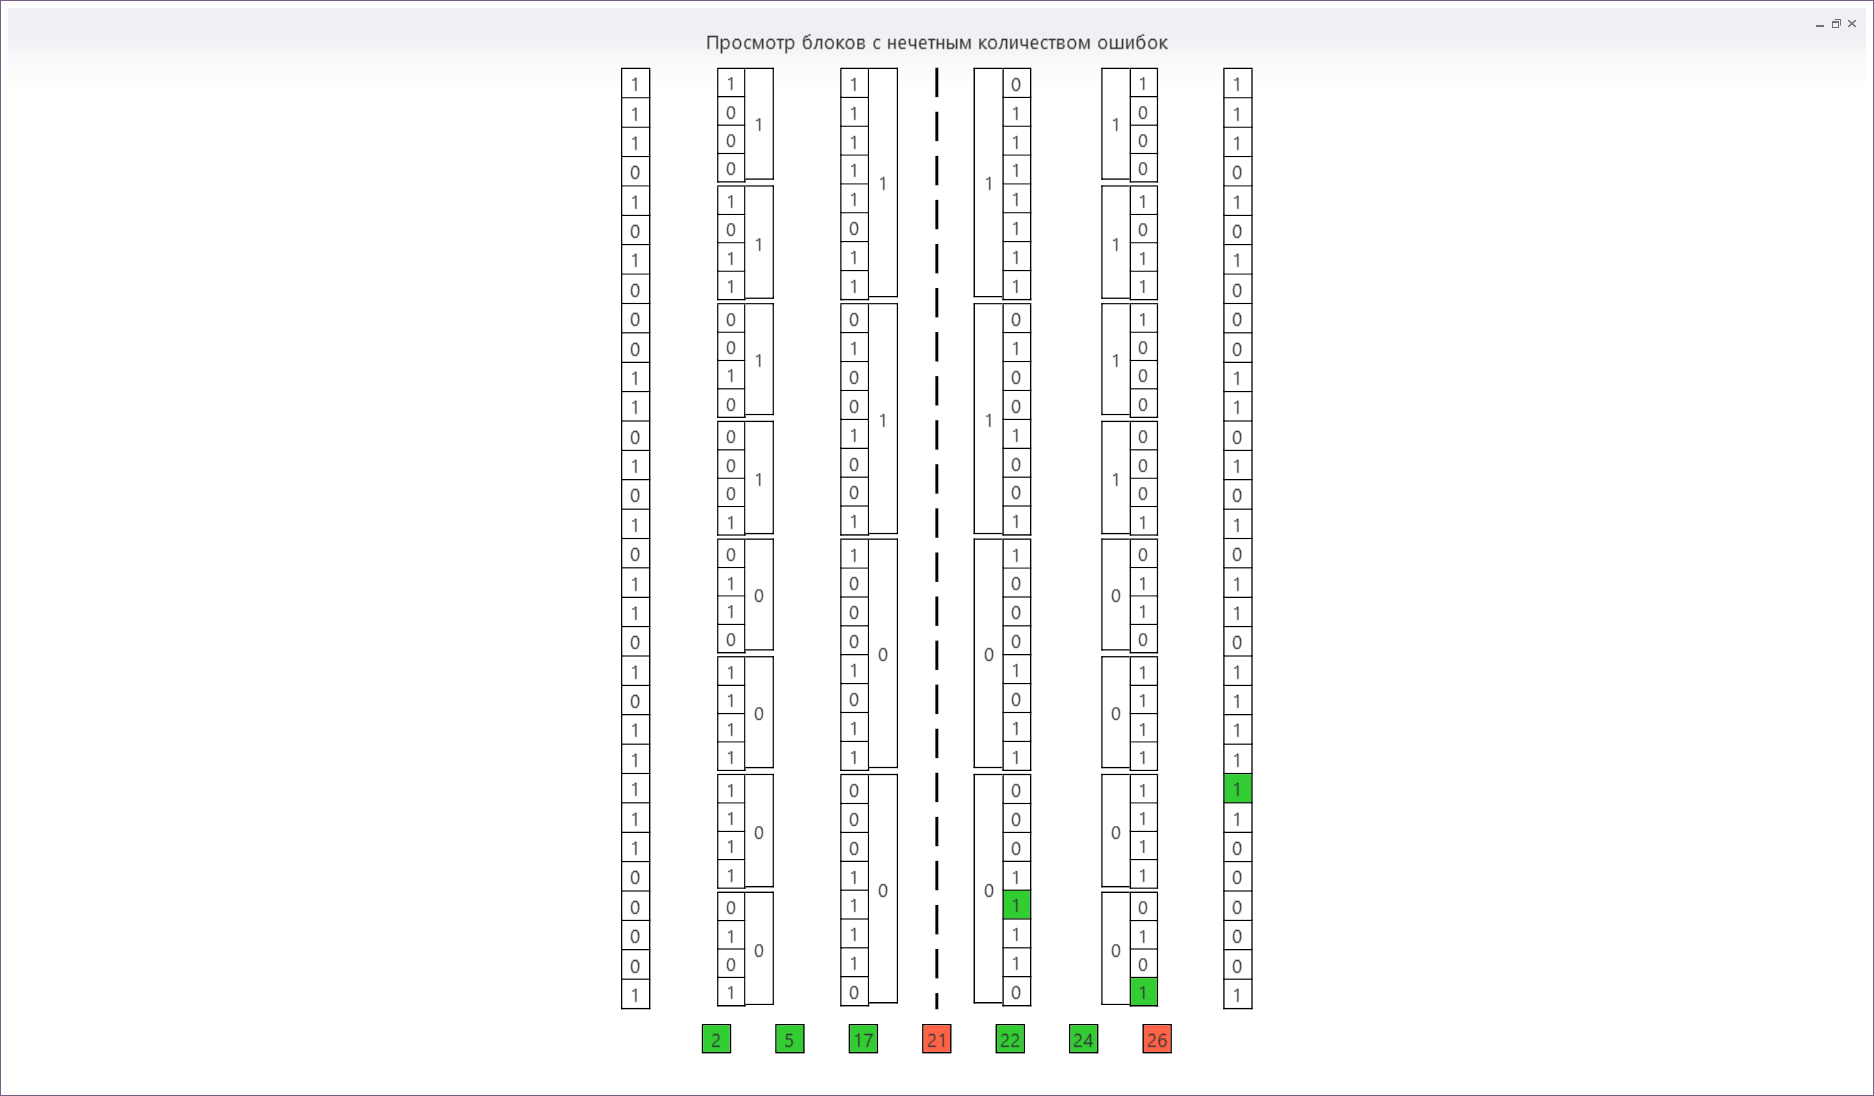
\includegraphics[width=0.9\linewidth]{chapter3/cascade_screenshots/16_error_backtrace}
  \caption{Все блоки, содержащие исправленную позицию и уже входящие в множество блоков с нечетным числом ошибок, удаляются из него.}
\end{figure}

\FloatBarrier
\begin{figure}[h]
  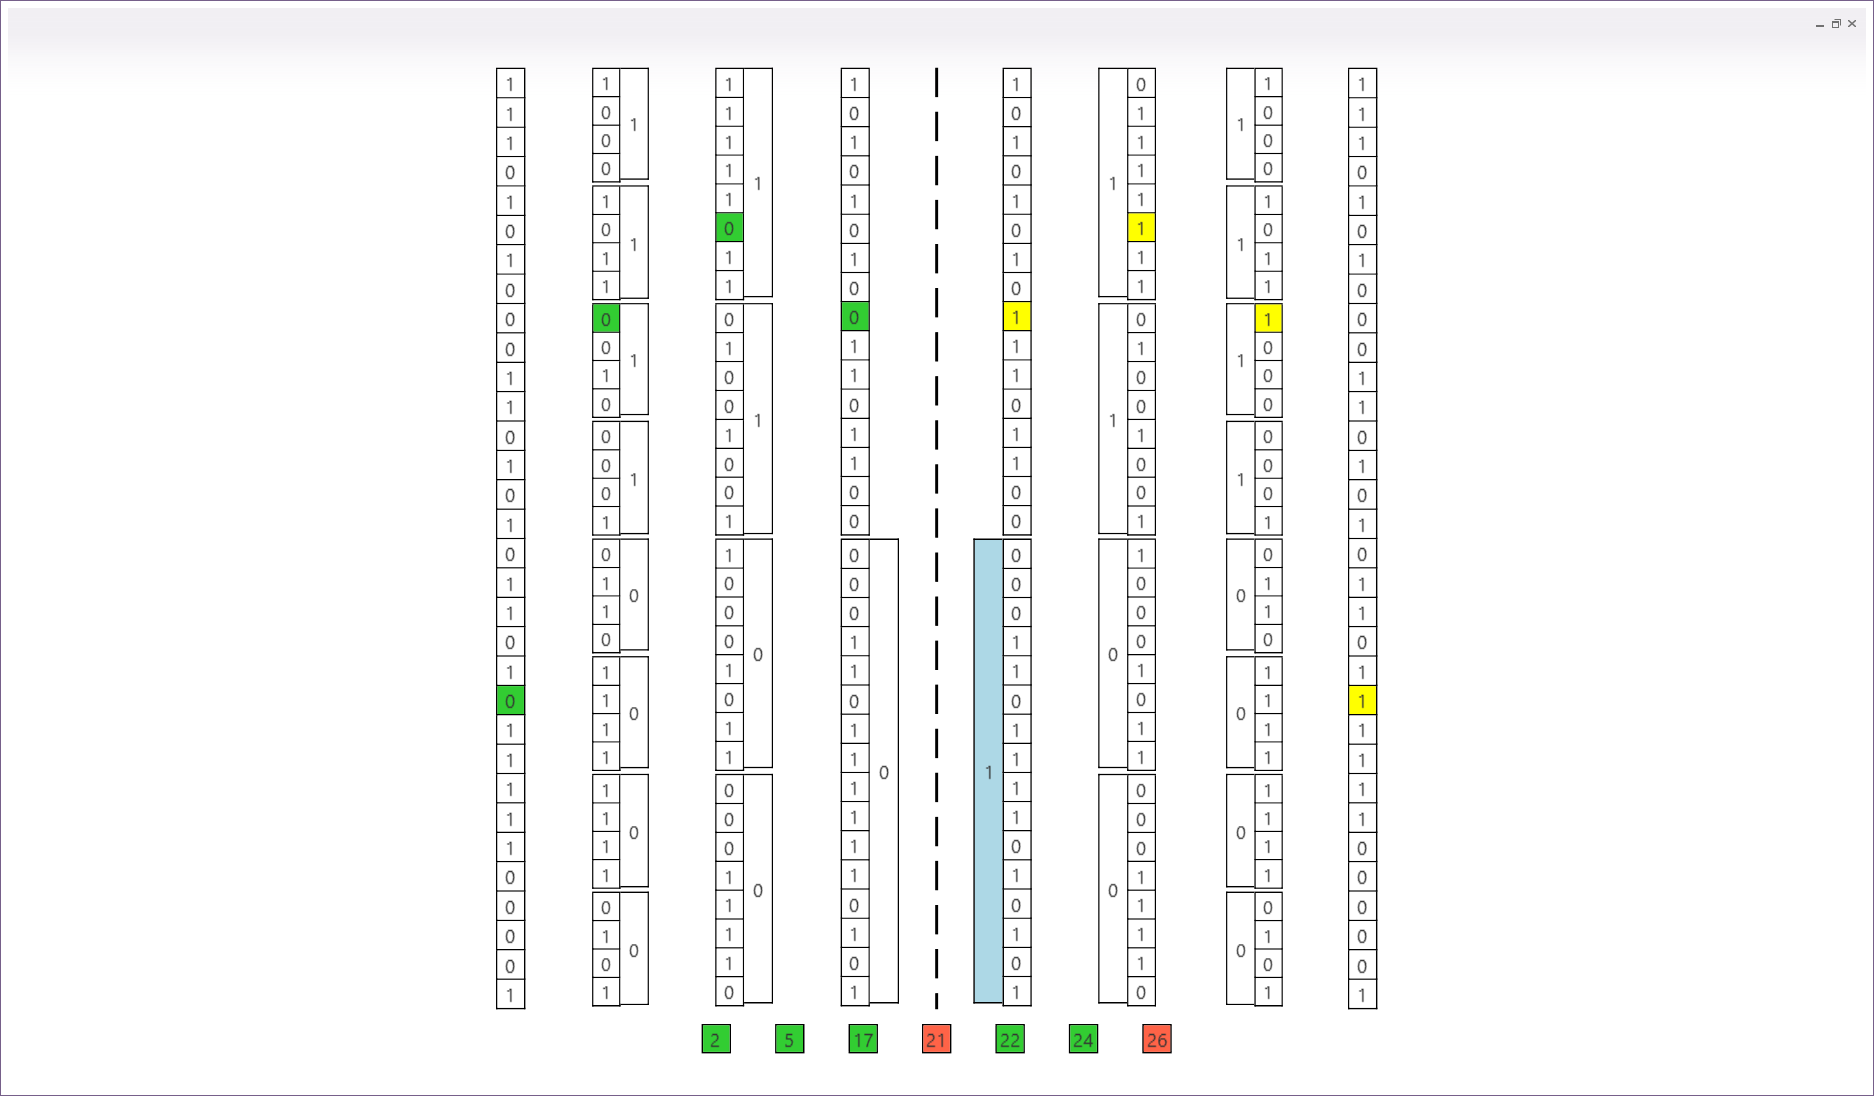
\includegraphics[width=0.9\linewidth]{chapter3/cascade_screenshots/17_error_found}
  \caption{Еще пример обратного распространения ошибки. Найдена ошибочная позиция в блоке на третьем проходе.}
\end{figure}

\begin{figure}[h]
  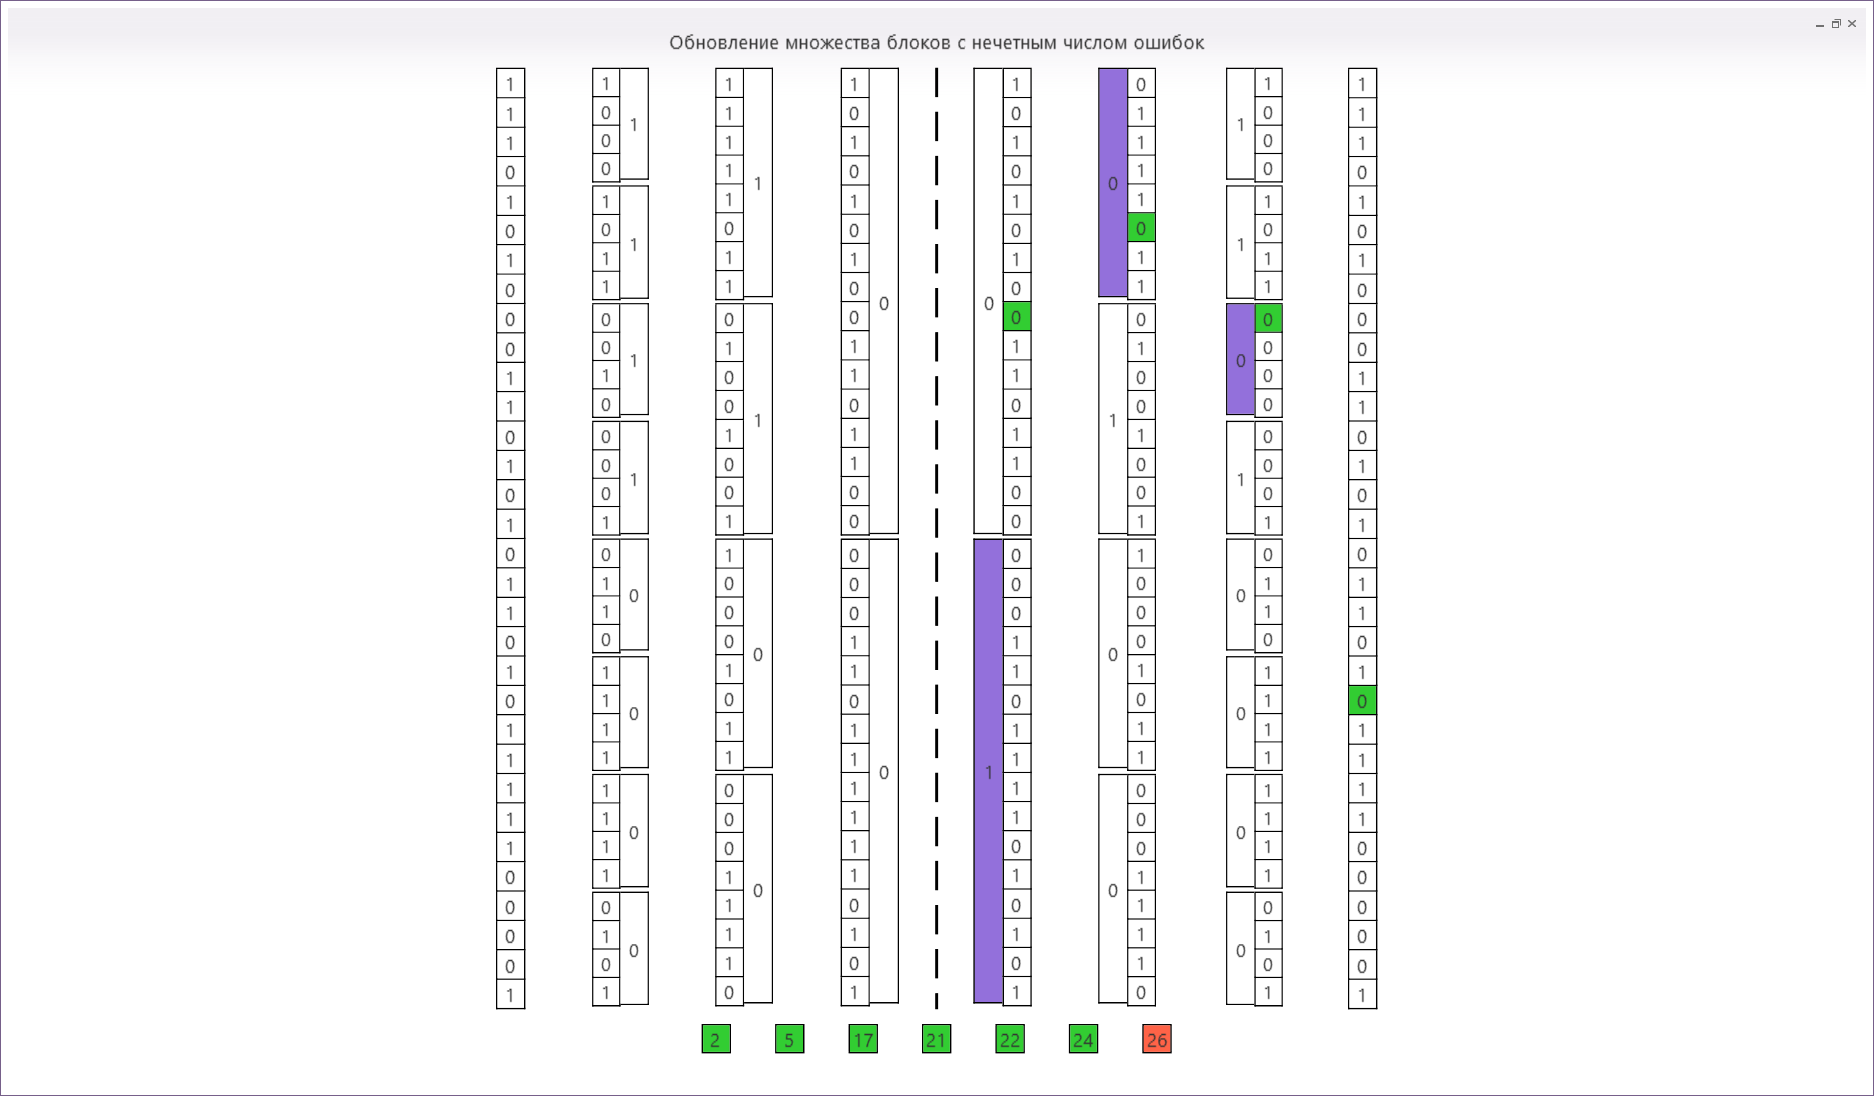
\includegraphics[width=0.9\linewidth]{chapter3/cascade_screenshots/18_error_backtrace}
  \caption{Блоки, содержащие исправленную позицию, вошли в множество блоков с нечетным числом ошибок.}
\end{figure}

\begin{figure}[h]
  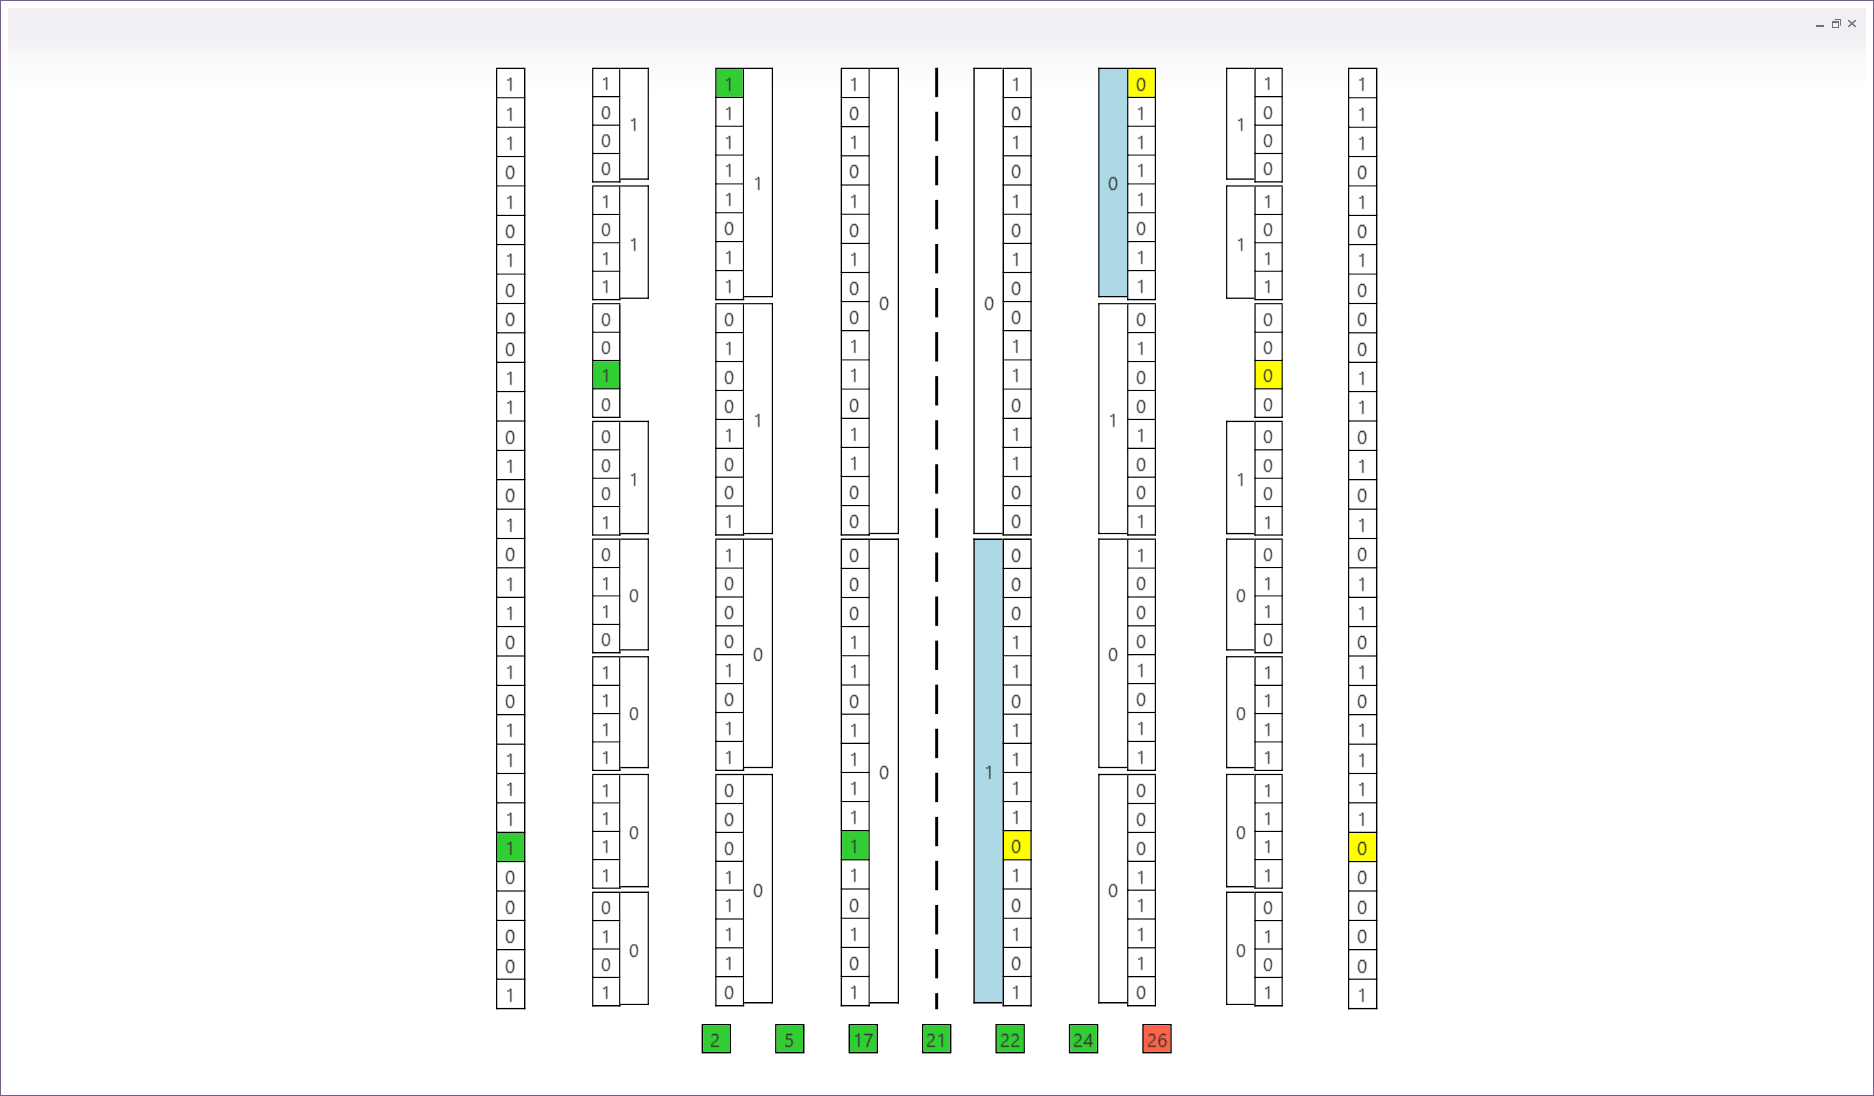
\includegraphics[width=0.9\linewidth]{chapter3/cascade_screenshots/19_error_found}
  \caption{В блоке наименьшего размера найдена последняя ошибочная позиция.}
\end{figure}

\begin{figure}[h]
  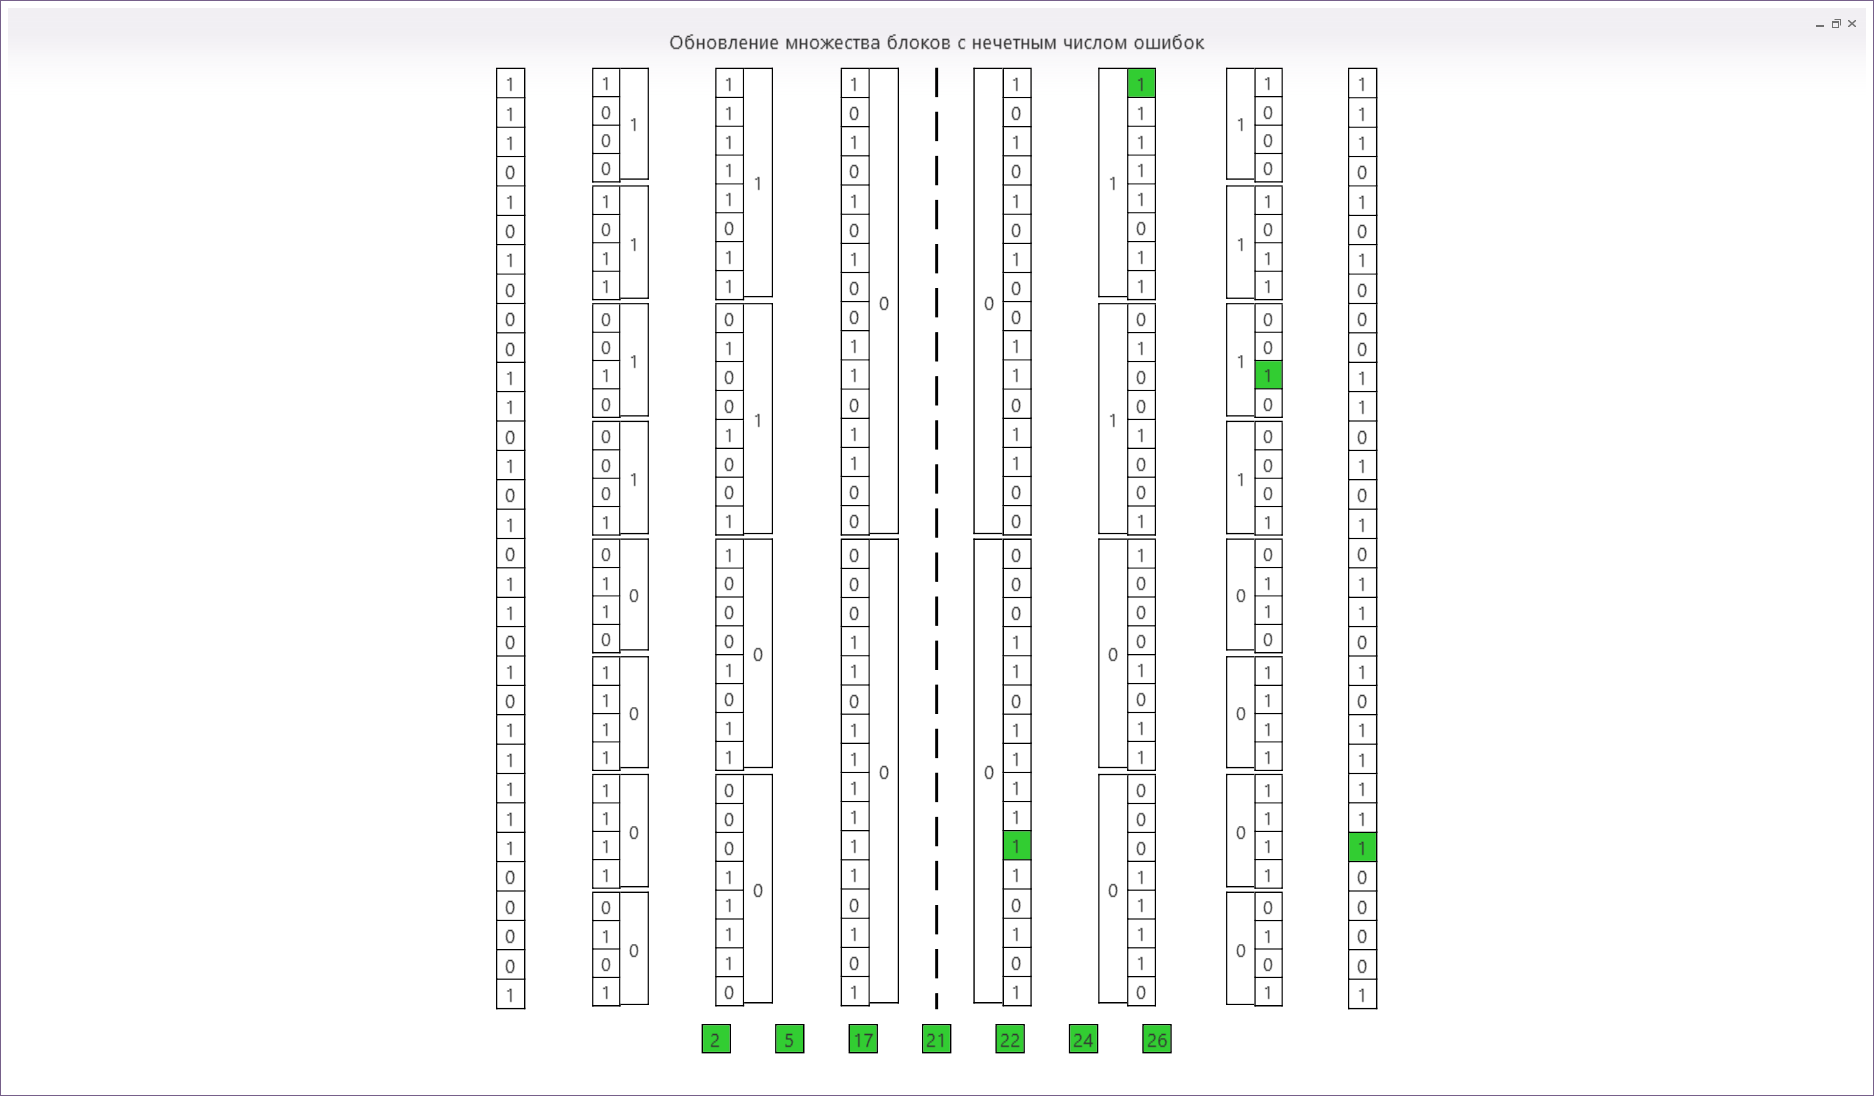
\includegraphics[width=0.9\linewidth]{chapter3/cascade_screenshots/20_error_backtrace}
  \caption{Блоки, содержащие исправленную позицию и уже входившие в множество блоков с нечетным числом ошибок, удаляются из него.}
\end{figure}

\begin{figure}[h]
  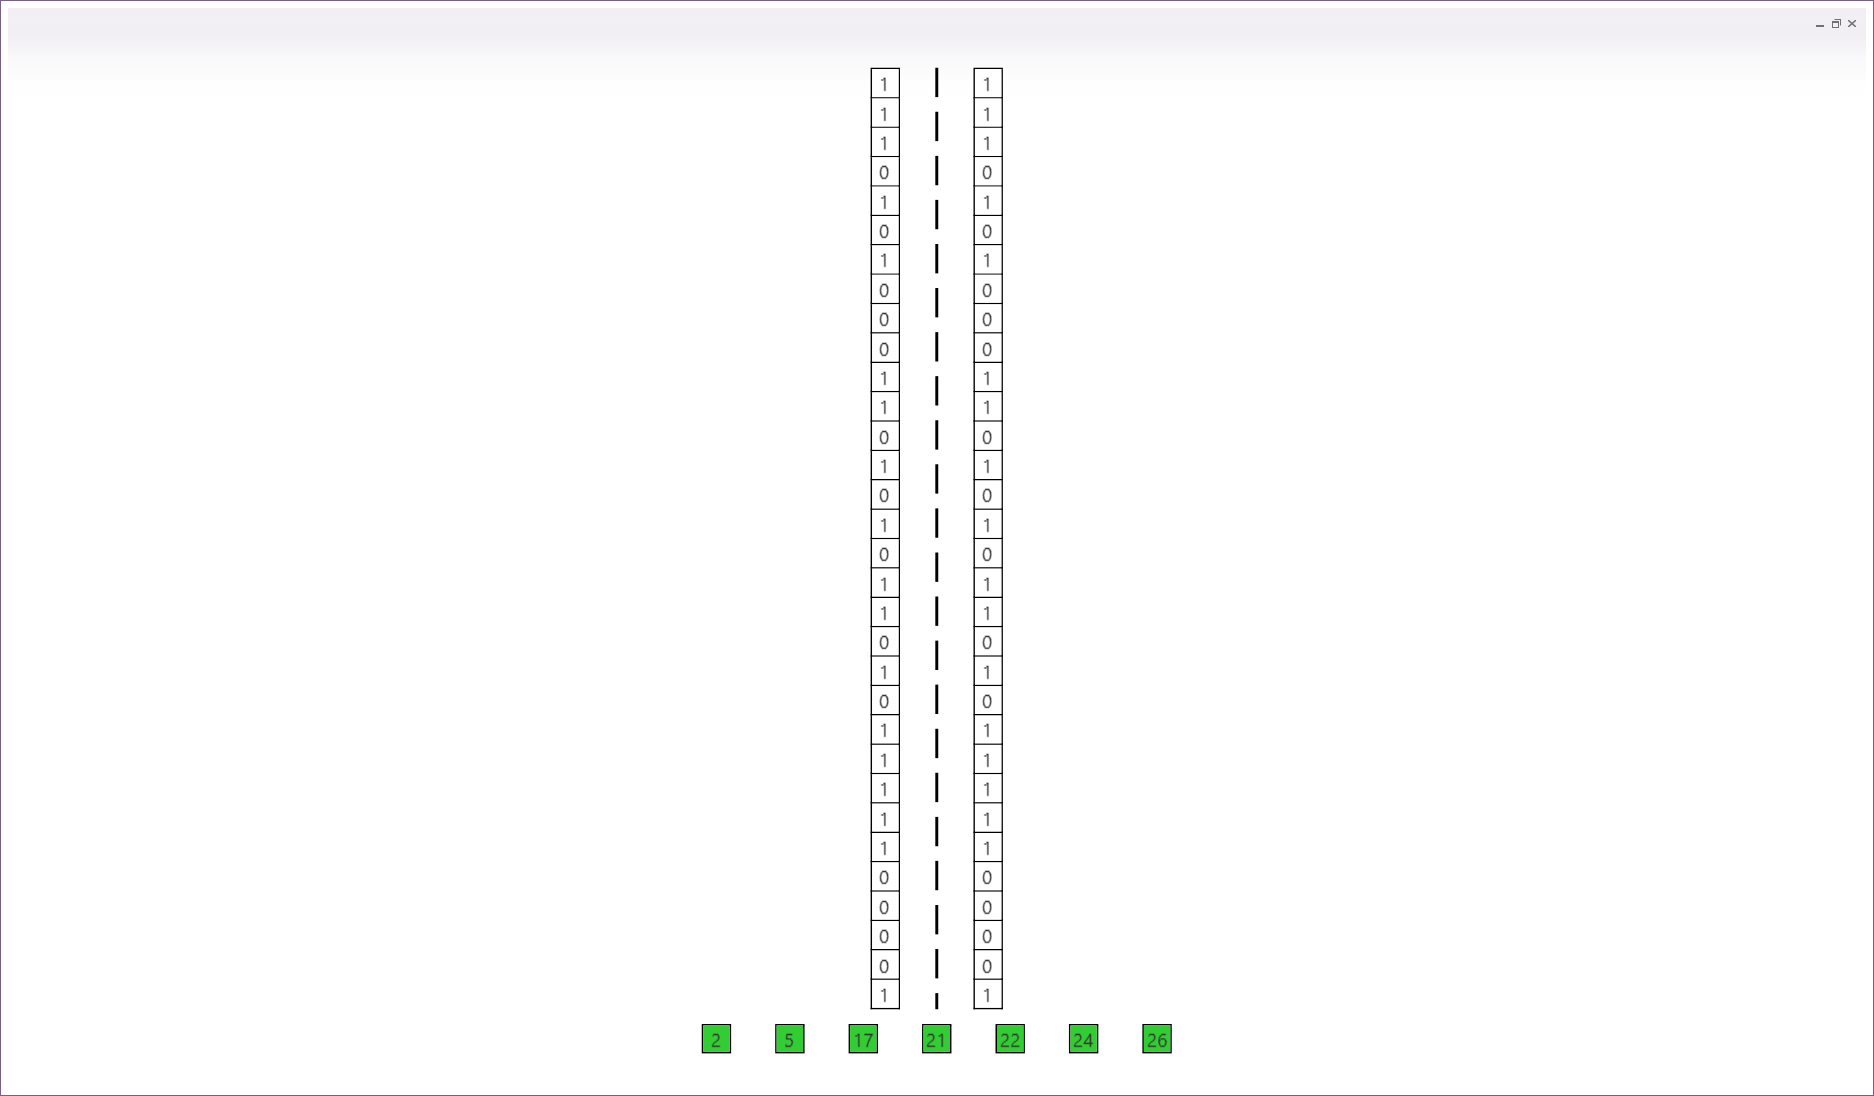
\includegraphics[width=0.9\linewidth]{chapter3/cascade_screenshots/21_end_state}
  \caption{Заключительное состояние программы. Все ошибки исправлены. Ключи сторон совпадают.}
\end{figure}
\clearpage